\documentclass[11pt, a4paper]{report}
\usepackage[left=40mm, right=20mm, top=20mm, bottom=20mm, includefoot]{geometry}
\usepackage{setspace}
\usepackage{titlesec}
\usepackage{graphicx}
\usepackage[english]{babel}
\usepackage[autostyle]{csquotes}
\usepackage{xcolor}
\usepackage{listings}
\usepackage{array}
\usepackage[toc, title, page]{appendix}
\usepackage{pdfpages}
\usepackage[style=apa, backend=biber, language=english]{biblatex}
\PassOptionsToPackage{hyphens}{url}\usepackage{hyperref}

\addbibresource{sources.bib}
\setlength{\parindent}{0ex}
\setlength{\parskip}{1.5ex}
\font\titlefont=cmr10 at 18pt
\MakeOuterQuote{"}

\titleformat{\chapter}[display]
  {\normalfont\huge\bfseries\flushleft\hyphenpenalty=10000}{\chaptertitlename\ \thechapter}{20pt}{\Huge}
\titlespacing*{\chapter}{0pt}{0pt}{40pt}

\lstset{
  frame=tb, % draw a frame at the top and bottom of the code block
  tabsize=4, % tab space width
  showstringspaces=false, % don't mark spaces in strings
  numbers=left, % display line numbers on the left
  basicstyle=\linespread{0.85}\selectfont,
  breaklines=true,
  postbreak=\mbox{\textcolor{red}{$\hookrightarrow$}\space},
  commentstyle=\color{olive}, % comment color
  keywordstyle=\color{blue}, % keyword color
  stringstyle=\color{red} % string color
}

\linespread{1.5}
\begin{document}


\includepdf[pages=-]{front_cover.pdf}

\title{\titlefont The path to the right decision: An investigation into using heuristic pathfinding algorithms for decision making in game AI}
\author{Ashley Rose}
\date{\today}
\maketitle
\thispagestyle{empty}

\renewcommand\abstractname{\textbf{Abstract}}
\begin{abstract}
The complexity and depth of video games are always growing, with AI being an important aspect of many modern-day games. Game AI has a variety of uses from being used as a plot device in a narrative game to being a replacement for human opponents in a competitive game, but the approach of choice for developing game AI is the traditional state machine. Many techniques such as behaviour trees aim to improve development to be more flexible and modular while being still being easy to implement. Pathfinding is a key element in the majority of these AIs; a decision would be made to navigate somewhere, and an algorithm such as A* is used to generate a path for the AI to follow to get to its destination. The problem with this is that there's no way of knowing if the destination can be reached and the way of getting there without pre-calculation. Moreover, information found when pathfinding, such as the destination being inaccessible, cannot be given back to the decision making system without restarting the whole process, occasionally resulting in unexpected behaviour.

This paper investigated how the pathfinding and decision making processes could be combined to make a new approach to game AI using the A* algorithm. Through substitution of types, A* can search a graph of data that isn't necessarily spatial to generate a sequence of actions to perform rather than locations to move to. Unfortunately, the testing of the prototypes made with this approach was hindered by problems caused by the amount of nodes being expanded and processed by A*. This, combined with the difficult methods for configuring the AI, ultimately meant that the AIs created for this paper would be unsuitable for non-academic use-cases unless the problems identified were solved, minimised or eliminated in some way.
\end{abstract}

\cleardoublepage
\setcounter{page}{1}
\pagenumbering{roman}
\tableofcontents

\cleardoublepage
\pagenumbering{arabic}
\setcounter{page}{1}

\chapter{Introduction}
\label{chapter:introduction}

\newcommand\invisiblesection[1]{%
  \refstepcounter{section}%
  \addcontentsline{toc}{section}{\protect\numberline{\thesection}#1}%
  \sectionmark{#1}}

\invisiblesection{Introduction}
\label{sec:introduction}

\subsection{Video games and artificial intelligence}
\label{subsec:videoGamesAndAI}

Games are good for the global economy. \citeauthor{Newzoo} \parencite*{Newzoo} reports that in October 2019 the global games market was worth \$148 billion. In order to remain competitive, developers are pushed to make bigger, better and more complex games. The evolution of the technologies available has allowed for a greater number of elements to be simulated in the game world which could potentially increase a game's worth \parencite{blow2004game}. The entry barrier to creating these good-looking and well-executed games has been lifted with the establishment of engines like Unity \parencite{Unity} and Unreal \parencite{Unreal} to the point where even non-programmers can get involved using textual or visual scripting.

For many years, only the game's graphics were considered important \parencites{yap2002grid, blow2004game}, however, good physics systems or competent AI (Artificial Intelligence) are now recognised as a way of improving the end-user's experience just as much \parencite{blow2004game}. Game AI is different from the normal, academic AI as it simulates behaviour and aims to be believable and fun, whereas an academic AI aims to achieve a level of intelligence or autonomy to excel at a given task \parencite[60]{nareyek2004ai}.

\subsection{The need for game AI}
\label{subsec:theNeedForGameAI}

AI has multiple uses within a games context but the majority of use cases employ AI to control the characters featured in a level of the game. \citeauthor{laird2001human} \parencite*[16]{laird2001human} said that whether these characters are replacements for opposing players or characters that act as companions, villains and plot devices, "human-level AI can expand the types of experiences people have playing computer games". Using AI opens up the opportunity for increasing the difficulty of the game, and could be perceived as the kind of challenges that make games fun \parencite[2]{buro2004call}. \citeauthor{laird2001human} \parencite*[16]{laird2001human} also hypothesised that utilising such an AI is a good step towards the development of enjoyable and challenging gameplay, and potentially to "completely new genres" \parencite[17]{laird2001human}.

"Customers value great AI" \parencite[60]{nareyek2004ai} and so it's important to choose a suitable approach that fulfils the expectations of the player thus the requirements of the game \parencite[19]{millington2019ai}. Academic AI can be made using algorithms inspired by biology such as neural networks or genetic algorithms and trained through iteration or with datasets. These approaches aren't used in game AI because of the high requirements to train the AI to interact with a specific game \parencite[64]{nareyek2004ai}, moreover, it is easy to train the AI to play too strongly ruin the game \parencite[13]{tozour2002evolution}. Instead, game AI developers embrace simpler, non-learning algorithms due to them being easier to understand, implement and debug \parencite[7]{tozour2002evolution}.

\subsection{Approaches to game AI development}
\label{subsec:approachesToGameAIDevelopment}

\begin{figure}[!h]
  \centering
  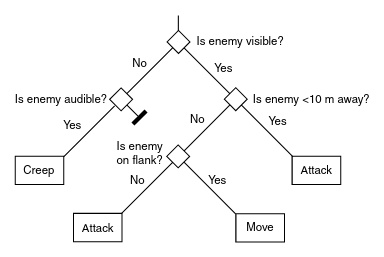
\includegraphics[width=10cm]{img/decision_trees.png}
  \caption{An enemy AI made with a decision tree \parencite[296]{millington2019ai}}
  \label{fig:decisionTree}
\end{figure}

The most basic forms of AI used in games take the form of a series of if-then statements and are known as `production rule systems' \parencite{tozour2002evolution}. These statements are organised in a list and the AI uses the behaviour of the rules that evaluate to $true$. The result is a very basic AI that is not only limited to what actions it can take but also when it can take them. Similarly, decision trees combine the same if-then style with branching structures to create game AI \parencite[62]{nareyek2004ai}, and the tree and subtrees are recursively traversed until a leaf node is found with the desired behaviour. This process is very easy to understand and implement \parencite[295]{millington2019ai}, and the branching structure makes visualisation of the process more intuitive than the basic list used in a production rule system. Because of this, many consider decision trees to be one of, if not the simplest techniques to making AI  (\cite[295]{millington2019ai}; \cite[7]{tozour2002evolution}). Figure \ref{fig:decisionTree} shows how a decision tree could be used for game AI.

\begin{figure}[!h]
  \centering
  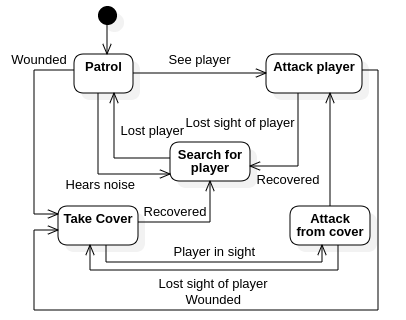
\includegraphics[width=10cm]{img/finite_state_machine.png}
  \caption{A guard's AI made with a Finite State Machine}
  \label{fig:finiteStateMachines}
\end{figure}

FSMs, or Finite State Machines, are the most common approach to game AI (\cite[1]{orkin2006three}; \cite[309]{millington2019ai}) due to being easy to understand and the efficacy of their output. As shown in figure \ref{fig:finiteStateMachines}, FSMs consist of a directed graph where each node represents a state and the edges represent the transitions between them \parencite[6]{tozour2002evolution}. A character can only be in one state at time and has no memory of any previous states \parencite{colledanchise2014performance}; each state represents an expected behaviour and determines what they do and the conditions to switch to a different state \parencite[3]{diller2004behavior}. In the right environment, the impression of a well thought out FSM could compete with that a neural network, at a fraction of the time and resource costs, despite not always arriving at the optimal decisions \parencite{sweetser2002current}. However, each new behaviour requires the creation of a new state and the conditions of which this state integrates and transitions into other states, making expansion and maintenance cumbersome (\cite[2]{sweetser2002current}; \cite[3]{lim2010evolving}). There's no easy way to combine the tests inside of FSMs and selecting the conditions for a state transition is still very much a process that must be done by hand \parencite[313]{millington2019ai}.

The need for more flexibility in game AI has lead to the creation adaptation of modular algorithms such as behaviour trees \parencite[1]{lim2010evolving}. Like decision trees, the recursive structure of a behaviour tree is simple to understand and implement while also being high level, allowing for more sophisticated AI to be created in a modular fashion through the use of subtrees and different node types \parencite[144]{shoulson2011parameterizing}, each performs an action or check and then proceeds to succeed or fail \parencite[4]{lim2010evolving}. It is these types that make the AI process at a higher level than standard decision trees, and when combined with leaf nodes that perform checks and actions to build trees, and then combined again to make trees containing subtrees, the simplicity and elegance of this technique certainly demonstrates why behaviour trees are getting attention \parencite[144]{shoulson2011parameterizing}. An example of a behaviour tree can be seen in figure \ref{fig:behaviourTree}.

\begin{figure}[!h]
  \centering
  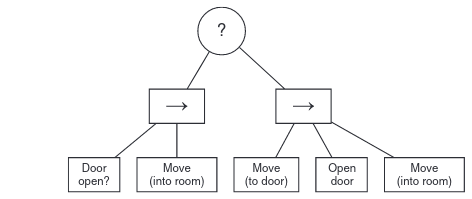
\includegraphics[width=12cm]{img/behaviour_trees.png}
  \caption{A behaviour tree for moving into a room \parencite[337]{millington2019ai}}
  \label{fig:behaviourTree}
\end{figure}

\subsection{The relationship of pathfinding and game AI}
\label{subsec:theRelationshipOfPathfindingAndGameAI}

One common requirement for game AI is for the characters to be able to traverse the areas of the game in a way which meets the player's expectations logically and efficiently --- a task known as pathfinding. Regardless of what an AI decides to do, a pathfinding mechanic needs to be in place to allow the AI to navigate to where it needs to go, manoeuvring around obstacles while still taking a sensible route \parencite[60]{graham2003pathfinding}. For most games, the algorithm of choice is A* as it is the de-facto standard pathfinding algorithm (\cite[197]{millington2019ai}; \cite[2]{botea2004near}; \cite[64]{nareyek2004ai}; \cite[73]{leigh2007using}).

The A* algorithm analyses the game's map and generates a path from one location to another while minimising a $cost$ value --- this value can represent anything but usually it represents the time or distance to travel along a given route \parencite[44]{yap2002grid}. This means that the pathfinding algorithm itself doesn't decide where to go, only how to get there and the manner in which it does so. When asked to calculate a path, a pathfinding algorithm is provided a graph of nodes to determine which nodes can be reached from which \parencite[61]{nareyek2004ai}. The algorithm isn't concerned in what the data represents (2D or 3D coordinate data), the data's form (a tree, a graph or a list of connections) or the unit of measurement to calculate the weight of an edge (length, traversal time or monetary cost), as long as it is equipped with the right functionality to digest this information (\cite[277]{millington2019ai}; \cite[60]{graham2003pathfinding}).

With the pathfinding process taking place after the decision has been made, the opportunity to involve the data gathered from pathfinding algorithm is missed. Often, the AI will decide to approach the nearest object, but obstacles in the way mean that the cost of navigating to the destination is greater than some alternative. While implementing the algorithm isn't difficult, ensuring the AI generates a path to the correct destination is difficult to do well \parencite{forbus2002qualitative}. Perhaps on the way to the destination, the character has to also navigate past traps or other hazards where it will need to decide whether to avoid or pass through --- decisions that A* isn't fully equipped to deal with on it's own. If the AI wanted to factor in these hazards and real cost values, it would have to perform a more advanced check on where to travel too, maybe even using the pathfinding algorithm multiple times to definitely make sure that it wants to take the generated path, potentially ruining the game's speed and overall performance.

Pathfinding algorithms are actually general purpose search algorithms applied to a spatial context (\cite[125]{cui2011based}; \cite[6]{orkin2003applying}; \cite[46]{yap2002grid}); there is no such restriction that these algorithms should be limited to pathfinding when in a games context. \citeauthor{millington2019ai} \parencite*[197]{millington2019ai} said that "pathfinding can also be placed in the driving seat, making decisions about where to move as well as how to get there". With search algorithms having the flexibility of being able to traverse graphs of nodes representing any kind of data, it's no stretch to imagine the A* search algorithm being applied to a graph containing the same tests and actions found in decision and behaviour trees in order to generate a `path' of actions rather than a path of spatial data \parencite[114]{higgins2002generic}. This is paper aims to investigate and re-engineer A* to make decisions rather than paths in a game context.

\section{Literature Review}
\label{sec:literatureReview}

\subsection{Dijkstra's algorithm: A graph and tree search algorithm}
\label{subsec:dijkstrasAlgorithm}

A search algorithm is a recursive method designed to find a match for a piece of data within a collection such as an array, graph or tree \parencite{friedman1976algorithm}. A piece of data is provided and the search algorithm typically returns whether it is present and it's location. \citeauthor{dijkstra1959note}'s algorithm \parencite*{dijkstra1959note} is a search algorithm that operates on trees and graphs (which are then interpreted as trees). The algorithm calculates the shortest difference from any node on the graph to any other node, and can be terminated early to avoid unnecessary computation if a destination is provided and found.

\begin{figure}[!h]
  \centering
  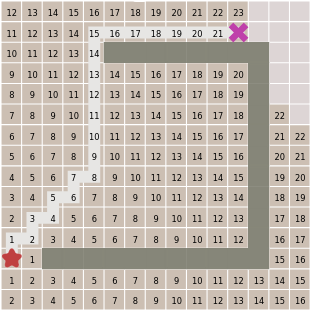
\includegraphics[width=8cm]{img/dijkstras_algorithm.png}
  \caption{Dijkstra's algorithm \parencite{red2014introduction}}
  \label{fig:dijkstrasAlgorithm}
\end{figure}

Dijkstra's algorithm works through the recursive summation and comparison of distance values starting from the a given start node \parencite[269]{dijkstra1959note}. Each neighbouring node is added to the \emph{open} list, then, the current node's distance from the start is added to the length between the current node and its neighbour. If this tentative value is lower than the current distance value of the neighbour, it replaces it. When all the neighbours have been considered, the node with the lowest tentative value on the graph is selected and permanently `visited' and are removed from the \emph{open} list \parencite{dijkstra1959note}. This process is repeated until either there are no \emph{open} nodes left or the destination, if provided, has been visited, and thus a path and the distance from the start to the destination can be retrieved. The problem with Dijkstra's algorithm is that it always selects the node with the lowest tentative distance value, meaning that the algorithm has no notion of direction and is calculating the lowest distance to nodes that may not be relevant to getting to the destination \parencite[214]{millington2019ai}. Figure \ref{fig:dijkstrasAlgorithm} illustrates how Dijkstra's algorithm expands the closest nodes until the goal has been found.

\subsection{A* algorithm: A heuristic best-first search algorithm}
\label{subsec:aStarAlgorithm}

A* is an improvement of Dijkstra's algorithm in this regard \parencite[101]{hart1968formal} --- while it doesn't stray far from how Dijkstra's algorithm works in the sense that it operates using a tentative distance value and it keeps track of the nodes that have and haven't been visited, it does extend the algorithm using what's known as a heuristic approach \parencite[126]{cui2011based}. "Heuristics are criteria, methods or principles for deciding which among several alternative courses of action promises to be the most effective in order to achieve some goal" \parencite[3]{pearl1984heuristics}. This means that in a pathfinding situation, a heuristic function could estimate the distance to the goal, by ignoring walls and measuring in a straight line, to direct the algorithm in the right direction and avoid evaluating routes that travel in the wrong direction to make the process more efficient \parencite[127]{cui2011based}. Heuristics enable A* to perform a best-first search \parencite[46]{yap2002grid}, as the heuristic now has the power to select which node is the best to evaluate and prioritise over the others \parencite[94]{russell2016artificial}.

When identifying the next node to expand, A* will take this heuristic distance into account using the formula $f(n) = g(n) + h(n)$ (\cite[102]{hart1968formal}; \cite[95]{russell2016artificial}), where $g(n)$ is the real distance the algorithm has calculated from the start node to node $n$ and is the distance to be minimised while finding the \emph{goal}, $h(n)$ is the \emph{heuristic} distance from the current node $n$ and the destination, and $f(n)$ is the combination of these two metrics forming an estimate of the distance from the start node to the destination if travelling through node $n$, also known as the \emph{fitness} value (\cite{hart1968formal}; \cite{millington2019ai}; \cite[64]{graham2003pathfinding}). Figure \ref{fig:aStarAlgorithm} shows how a heuristic function can guide the A* algorithm to avoid exploring nodes that aren't effective for navigating to the goal.

\begin{figure}[!h]
  \centering
  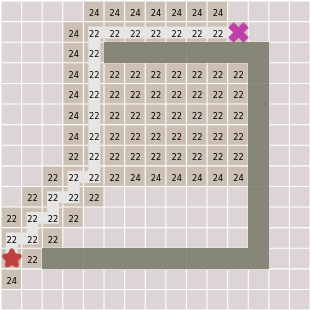
\includegraphics[width=8cm]{img/astar_algorithm.png}
  \caption{The A* algorithm \parencite{red2014introduction}}
  \label{fig:aStarAlgorithm}
\end{figure}

This heuristic component of A* transforms it into a family of algorithms where applying a different heuristic selects a different algorithm \parencite[107]{hart1968formal}, moreover, implementing A* and using a heuristic that returns a constant value for all nodes reverts A* back into Dijkstra's algorithm (\cite[10]{lester2005pathfinding}; \cite[237]{millington2019ai}). Conversely, implementing a well-designed heuristic method can be used to guarantee optimal solutions, and using a heuristic that is somewhere in-between can output results with varying degrees of accuracy in exchange for faster execution \parencite[219]{millington2019ai}.  The implementation of a good heuristic can be difficult, as making the heuristic take more factors into account for accuracy has the drawback of making the algorithm less efficient overall with the heuristic being frequently used throughout the process.

On the other hand, \citeauthor{graham2003pathfinding} \parencite*[68]{graham2003pathfinding} argue that one of the constraints of games the industry is the "over-reliance" on the A* pathfinding algorithm and describe the development of its many extensions as a way of avoiding the discovery of new techniques. The pathfinding process can require a lot of CPU resources, sometimes to the point of stalling the game, when applied to larger graphs (\cite[127]{cui2011based}; \cite[110]{stentz1996map}; \cite[67]{graham2003pathfinding}). This indicates that the performance of A* can vary depending on various factors, and is why it is important to optimise A* by selecting an suitable storage mechanism for the graph and internal node storage as well as using a reasonable heuristic that balances efficiency and efficacy \parencite[228]{millington2019ai}.

\subsection{Processing a character's perception of the game world}
\label{subsec:processingACharactersPerception}

These approaches need a way to digest information about the character and its environment that is relevant to the decision making process, and the selection of this information is just as important as the form it is delivered in \parencite[126]{cui2011based}. This extraction of world data can vary in difficulty \parencite[3]{diller2004behavior} and is done for both performance and gameplay needs. All game AI solutions need the world to be re-interpreted to be better suited for both decision making \parencite[2]{buro2004call} and pathfinding \parencite[3]{diller2004behavior}. Particular geometry of the map may need to be interpreted as vantage points, choke points or safe spots; particular formations of enemy units may need to be not only counted but also assessed for tactical strengths, whether engaging the units head-on is better than running away to a better location, and finally, the interpretation of time such as whether there is enough time to navigate to what would otherwise be a better location for fighting the enemy \parencite{buro2004call}. An AI would then take this abstraction of the world, combine it with the character's data and then consider what the character should be doing --- if the character is in an `attacking' state and the player is nearby then the decision would involve getting into a position and hitting or shooting at the player.

If A* is to be used for game AI it will need to operate on non-positional data. In standard pathfinding, each node is a position in the world and the edges between these nodes are the movements to get from one to another. Substituting each node to be an AI state and each edge to be an action that changes a state creates a graph that A* could process. The implementation the states and actions depend on the expectations of the AI --- traditional pathfinding could be implemented by having an action that triggers movement and changes the position variable in the character's state. Regardless, a graph consisting of these nodes could be difficult to process and reduce the speed of A*.

A* can suffer from performance problems when used with many agents at once, or with a large or inefficient graph of nodes \parencite{graham2003pathfinding}. Many solutions have been discovered to prevent or reduce the impact on performance --- one such solution is known as hierarchical pathfinding, where the game's map is simplified into chunks \parencite[126]{cui2011based}. Figure \ref{fig:hierarchicalPathfinding} shows how the pathfinding process can be applied to larger or more complex worlds; large groups of nodes can be simplified and reduced to singular nodes that represent their corresponding group \parencite{botea2004near}, similar to how quadtrees work. This works well for standard pathfinding, but if A* is applied to something other than purely spatial world data then the nodes need extra consideration.

\begin{figure}[!h]
  \centering
  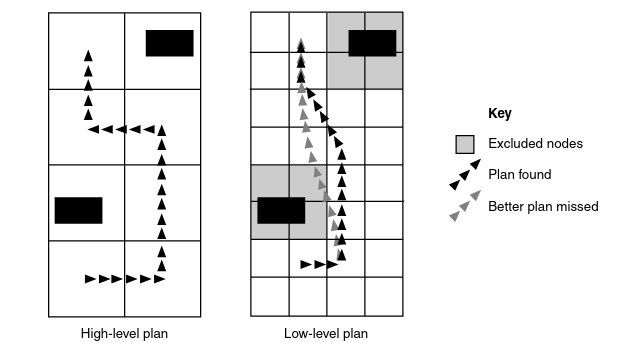
\includegraphics[width=\linewidth]{img/hierarchical_pathfinding.png}
  \caption{Hierarchical pathfinding \parencite[263]{millington2019ai}}
  \label{fig:hierarchicalPathfinding}
\end{figure}

There is a large amount of actions a character can take at any given moment \parencite[62]{nareyek2004ai} and so applying a search algorithm to such a large set of tasks will make the process a lot slower than traditional methods if left unchecked. Hierarchical pathfinding essentially creates more nodes to expand in the short term to reduce the total number of nodes expanded in the long term and gain a net increase in performance. Hierarchical pathfinding reduces the amount of destinations by collecting connections between the nodes in a given area and simplifies navigation to and from this area. This technique would be applicable to the character's state so long as these connections can be aggregated using other metrics other than purely relying on their proximities to each other. One such way of grouping  could be separating `attacking' actions from `defending' actions so that characters deciding to play defensively can safely ignore groups of related nodes. Splitting gameplay elements like this can get complicated --- if a certain unit in a strategy game can attack from a longer range, would attacking the enemy from a distance be a defensive manoeuvre or an offensive one, and how easy is this to change on a per-unit basis \parencite{weber2011building}?

\subsection{Making decisions with A* using GOAP}
\label{subsec:makingDecisionsWithAStarUsingGOAP}

\citeauthor{orkin2003applying} \parencite*[11]{orkin2003applying} expressed that expectations of AI are growing with the release of every new game and that "we need to look toward more structured, formalized solutions to creating scalable, maintainable and re-usable decision making systems". Techniques used to create the Game AI featured in most games do not contain the scalability \citeauthor{orkin2003applying} envisions \parencite[17]{laird2001human}, however, \citeauthor{higgins2002generic} \parencite*[117]{higgins2002generic} declares that a pathfinding engine can be created generically, especially if a templated language is used, to give the code even more reusability. Implementing A* in this way would allow it to be used for both regular pathfinding and anything else that could requires searching \parencite[120]{higgins2002generic}. With A* being efficient and optimisable \parencite[215]{millington2019ai}, reusing A* for game AI has the potential to bring the benefits it usually brings to pathfinding to AI while being adaptable enough to scale up and meet expectations.

\citeauthor{orkin2006three} \parencite*[1]{orkin2006three} worked on the development of the game AI for the game F.E.A.R \parencite{FEAR}. The approach used for this AI was called GOAP which stands for `Goal Oriented Action Planning' and uses the A* algorithm as part of its decision making process and "allows characters to decide not only what to do, but how to do it" \parencite[1]{orkin2003applying}. GOAP changes the data to be processed by A* from spatial data such as coordinates into character AI state data, such as what is found in FSMs. Therefore, the output of A* is no longer a sequence of movements but a sequence of actions also known as a plan (\cite[2]{orkin2003applying}; \cite[6]{tozour2002evolution}).

GOAP essentially takes the idea of having state machines to encapsulate behaviours and replaces the hand-programming the conditions and connections of state transitions with a pathfinding process with the aim being the decoupling of states and their transitions \parencite[2]{orkin2003applying}. The pathfinding process uses each node to represent a state and the edges between each node as the actions that lead to those states \parencite[7]{orkin2003applying} When GOAP is used, a goal is given for the character to achieve, which drives the AI to play the game rather than idly remain inactive, and what is returned is the sequence of actions that will satisfy the goal \parencite[1]{orkin2003applying}. An action is a representation of one thing the character will do to change the world in some way, like opening a door or picking up a weapon \parencite{orkin2003applying}; some actions have preconditions that require the execution of another action prior to it \parencite[5]{orkin2003applying}. A* will then find the sequence of actions, the plan, that satisfies the character's goal while minimising an arbitrary $cost$ value --- \citeauthor{orkin2003applying} \parencite*[4-5]{orkin2003applying} suggests that this process creates interesting character AI that can adapt to change while also having a code structure that is reusable, maintainable and "elegant".

\begin{figure}[h]
  \centering
  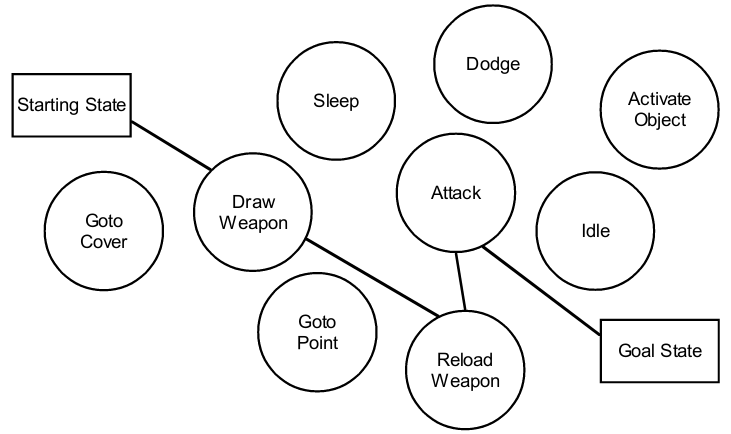
\includegraphics[width=12cm]{img/goap.png}
  \caption{An example of GOAP \parencite[3]{orkin2003applying}}
  \label{fig:goap}
\end{figure}

A* being used in GOAP means that fundamental formula $f(n) = g(n) + h(n)$ \parencite[102]{hart1968formal} is implemented in a way such that A* can perform a best-first search and expand the actions that are more likely to be  useful to the situation \parencite[7]{orkin2003applying}. To calculate $h(n)$, \citeauthor{orkin2003applying} \parencite*[7]{orkin2003applying} also shares that the heuristic in GOAP can be calculated as the summation of unmet conditions of the goal node, but this is rather unclear. Given the example in figure \ref{fig:goap}, "the goal is to kill an enemy" \parencite[3]{orkin2003applying} could be interpreted in various ways that all seem unsuitable. If the goal condition is that the enemy is dead, the heuristic would be the same for all nodes but the goal state, making it potentially wasteful like Dijkstra's algorithm \parencite[214]{millington2019ai}. Alternatively, if the condition was divided into multiple conditions such as the weapon needing to be drawn, the weapon needing to be loaded, and the enemy being dead, it is implied that either the algorithm has been run previously to determine the requirements of killing an enemy, or that they were programmed by the programmer --- how would the starting state know that the weapon needed to be reloaded before drawing it? While GOAP does seem elegant, the graph in figure \ref{fig:goap} doesn't have a sizeable number of nodes; using Dijkstra's algorithm wouldn't incur much of a performance cost with a graph this size. \citeauthor{orkin2003applying} \parencite*{orkin2003applying} suggests that a regressive search by starting at the goal and pathing to the start makes sense, and in figure \ref{fig:goap}, it does, as only one action can attack and so it's clear that the decision making process boils down to the character attacking the enemy.

Another problem of GOAP is that the high-level nature of the approach may not allow for enough control of the game \parencite[87]{stanciu2012implementing} --- while making abstractions of the world is necessary for AI to process the information \parencite[2]{buro2004call} and thinking on a higher level is beneficial for making more human-like decisions, the precision of the actions taken by the AI is both low level and very noticeable if incorrect \parencite[60]{graham2003pathfinding}. Figure \ref{fig:goap} shows a decision making process that decides what to do but not necessarily where to do it. When the action "Goto Point" in figure \ref{fig:goap} gets executed, there's no indication of how the destinations are generated other than satisfying the preconditions for another action (for example, moving to an object to activate it) \parencite[7]{orkin2003applying}.

This isn't specific to GOAP as it applies to every AI approach where the generation of these locations isn't part of the AI. Is the character's AI deciding where to go, or just deciding that it has to go somewhere? In order for "Goto Cover" to act in a similar way to the "Goto Point" action, a goal or action precondition would either have to require the character to be out of line-of-sight, or be using one of the designated cover spots --- this is how F.E.A.R \parencite*{FEAR} approached it \parencite[12]{orkin2006three}. The former would require calculating the closest position that allows the escape of line-of-sight. The latter of these would require set locations to be marked as points of interest and then A* would be employed to find which cover spot would be the quickest to navigate to. Both of these would have their own problems, and wrapping the entire pathfinding process as a single action would mean that the information from the pathfinding request would not be used in the decision making at all. Without utilising the AI's ability to create an impression of thought, the information given to these actions could be poorly chosen and "may be perceived as a lack of intelligence by a human player" \parencite[63]{graham2003pathfinding}.

\subsection{Defining the notion of cost in the context of game AI}
\label{subsec:definingTheNotionOfCost}

Cost, sometimes referred to as weight, is a term that will continue to be used when talking about A* as it is the the metric that governs the searching process \parencite[60]{graham2003pathfinding}. Cost doesn't have to be a numeric value, as long as it can be compared and combined correctly with other cost values. However, one numeric restriction of cost is that it cannot, or rather should not, be negative. The method A* uses to determine if a route should be expanded before another is if its cost value is lower --- when only positive values are added together it is assumed that costs cannot decrease in value. While in mathematics it is entirely possible and valid for these values to be negative, the problems that make this necessary are not applicable to games \parencite[202]{millington2019ai}.

In the formula $f(n) = g(n) + h(n)$ \parencite{hart1968formal}, each function returns a cost --- the combination of the goal and heuristic cost values, also known as the fitness value, is used select the next open node to evaluate \parencite[94]{russell2016artificial}. If $a$ and $b$ are two nodes in a graph and $f(a) < f(b)$, A* will interpret this as node $a$ being a more logical choice to expand \parencite[7]{orkin2003applying}. Node $b$ won't be evaluated unless the routes derived from node $a$ are dead ends or have worse fitness values than node $b$. With the order of execution being so dependent on $f(n)$, it is important that the definition of the cost of an action is calculated correctly. It is difficult to design such a system when everything is arbitrary, but metrics such as distance can be used to prioritise actions with lower distances such as movement, resources such as gold or mana could be used in game specific interactions to minimise spending important resources, and the time spent doing the action can also be factored in to drive the character to resolve the situation as quickly as possible \parencite[8]{lester2005pathfinding}. \citeauthor{millington2019ai} \parencite*{millington2019ai} said that "the cost function is a blend of many different concerns, and there can be different cost functions for different characters in a game" and that this is called "tactical pathfinding". The ability to change the cost per character further demonstrates the adaptability of A* --- changing the way a character interacts with the world is just changing these cost functions so that the A* prioritises one action over another.

Some decisions are more troublesome to weigh than others; with the constraint of non-negativity, what would the cost be of an ability that regenerates mana instead of expending it? The only way to apply reductions to values in this way would be to have a baseline cost for an action and then add or subtract from it, however, this does mean that this baseline value would dictate the maximum value of the reduction and so forward planning is necessary to ensure that all reductions can be applied in a balanced way. Another difficult type of decision to way are ones that don't have inherent characteristics; with a good goal for AI being unpredictable, surprising behaviour \parencite[17]{scott2002illusion}, how would the incentive for performing strategies like flanking and ambushing be created, and how would it compare to the cost for attacking an enemy directly head-on? \citeauthor{orkin2006three} \parencite*[14]{orkin2006three} said that in F.E.A.R \parencite{FEAR} this behaviour just came naturally from using a dynamic decision making system such as GOAP and that while they were prepared to implement "complex squad behaviour", none was implemented --- the squad's ability to ambush "emerged" from the combination of the "squad level" decisions and the individual character's decisions which gave the illusion of complex behaviour. \citeauthor{orkin2006three} doesn't mention much more on this subject and so GOAP's ability to surprise remains uncertain.

\citeauthor{harmon2002economic} \parencite*[405]{harmon2002economic} suggests that an "opportunity cost" could be introduced which represents the other actions that cannot be taken as a result of taking the given, mutually exclusive action, the objective being to consider alternative and potentially better courses of action that are available when applying penalties to actions. While it is difficult to reward the AI for executing good strategies, applying opportunity costs to other actions could get complex in both design and implementation; there is no discussion of this concept from \citeauthor{orkin2006three} \parencite*{orkin2006three} from his work on F.E.A.R and it is unclear how \citeauthor{harmon2002economic} applied these penalties. In order to calculate this opportunity cost, some component of the AI, such as the weighing function, needs to have knowledge of other nodes so that this cost can be determined and used, requiring further forward planning.

GOAP uses a simple "action cost" system to prioritise which tasks to carry out first \parencite[11]{orkin2006three}. Using an integer or floating point value is ideal for the type of cost as it can be added and compared with other values trivially. However, GOAP's method of creating unique characters is to assign unique sets of actions to make them act differently \parencite[8]{orkin2006three} as opposed to giving them alternative ways of evaluating situations as \citeauthor{millington2019ai} \parencite*{millington2019ai} suggested. Giving characters different actions will implicitly change how they prioritise the same situation as they will be given new routes to explore, and for most games this might be the best idea. It could be a good idea to split the cost type into a set of values to give actions different values. Throwing a grenade and shooting a pistol could be considered equivalent in difficulty to perform, but typically grenades have more firepower in exchange for there being less available; reducing these actions to a single value could be difficult depending on the approach, but splitting the value into a set would allow the programmers to keep track of firepower and usage penalties separately. When needed for comparison, this set would evaluate to the sum of it's parts --- but certain characters or situations could choose to adjust or completely omit parts of the cost so that actions are perceived in different ways depending on how a character views a certain cost. For a fast character, the cost to move might be halved and the cost of being exposed doubled in order to give the impression of an agile and hard-to-hit character.

\subsection{Generation, selection and application of goal state nodes}
\label{subsec:generationSelectionAndApplicationOfStateNodes}

When the game world has been processed, the actions a character can perform have been laid out and the methods of evaluating courses of action have been provided, the only things remaining that A* needs to function are the start and goal node states for the actual decision. The starting state is trivial as it is simply the current state of the character and world; the goal state node requires more consideration than that though. In standard pathfinding, the output is the shortest path from the starting node to the goal node, if such a path exists \parencite[61]{nareyek2004ai}. For game AI though, the goal needs to represent how the character or world should be --- or rather the objective outcome of the decision making process. This objective can be difficult to ascertain as a goal node could represent anything; what seems to be a simple goal such `win the game' becomes a rigorous series of tests to both calculate the cost reaching the goal than another \parencite[403]{harmon2002economic}. On the other hand, objectives that are too small or disconnected may not combine correctly to form this over-arching goal of winning the game. A balance is needed, whether that means the objective is to chase the player or defend an area, the objective needs to be focused on winning without being vague.

While \citeauthor{orkin2003applying} \parencite*{orkin2003applying} talks about in great depth about how GOAP handles making a decision to satisfy goal conditions, he doesn't describe where these objectives come from. A "squad coordinator" is mentioned \parencite[13]{orkin2003applying} that organises multiple agents into squads when they're close together, but the actual goals of the AI can come from both the character's individual AI and the squad coordinator. GOAP doesn't replace an FSM, so it could be inferred that the character's state when a goal is reached determines the next goal and thus the character's behaviour, with the initial state being defaulted, scripted or randomised \parencite[2]{orkin2003applying}. Alternatively, game AI could be created in layers and the output of one layer could be the desired goal of another, but this just propagates the problem to the highest level layer.

Another talking point regarding goals is the amount of designated goal state nodes in the graph. There is typically only a single goal in standard pathfinding, but it is possible, maybe even advantageous, for some games to contain multiple goal nodes in a graph \parencite[272]{millington2019ai}. Instead of checking for a match with a certain location (or state, when developing AI), a method that checks whether a given node meets the requirements of being classified as a goal could be used instead; the heuristic would also need revision as it would need to calculate the heuristic cost to reach the 'nearest' goal rather than just the single, given goal \parencite[272]{millington2019ai}. Having multiple goals and goal types \parencite[121]{higgins2002generic} would grant the ability for the AI to re-route to a different goal if it's easier and therefore accomplish the same task in multiple different ways without creating generic goals; this has its drawbacks though, one being the need for a more intricate and potentially confusing implementation and design of the AI needs, the other being the creation of balancing difficulties to ensure goals are prioritised as expected.

\subsection{Summary}
\label{subsec:litReviewSummary}

Search algorithms such as A* are generic, maintainable and versatile and are therefore theoretically suitable replacements for FSMs and behaviour trees for implementing game AI. While GOAP does use A* for part of it's decision making process, it isn't a complete solution and still separates decision making from the pathfinding process. This is acceptable and valid as GOAP is for generating a sequence of actions whereas pathfinding is strictly for navigating the map in order to perform these actions. Unfortunately, some information found during pathfinding that could be considered useful for decision making is lost unless explicitly communicated --- a decision might request to navigate to some location, but the path generated might be longer than expected and a different course of action could have been more appropriate. Without replanning, GOAP's disconnect between these systems could result in the wrong decisions being made.

In this paper, the mechanisms of the A* search algorithm are examined and re-engineered, through the substitution of input and output types, to investigate the modularity and adaptability of an AI that uses search algorithms to make decisions while actively involving pathfinding in the process as opposed to keeping these systems separate. Several approaches to defining goals and heuristic methods will be used to visualise the effects they have on a squad-controlling game AI. The aim of using this approach is to bring decision-making and pathfinding closer together and therefore simplifying the overarching process of perceiving, deciding and interacting in the game world.

\section{Methods and Methodologies}
\label{sec:methodsAndMethodologies}

\subsection{Algorithm selection}
\label{subsec:algorithmSelection}

As discussed, this paper will be using A* as the pathfinding and decision making algorithm of choice. A* is already used in many games for pathfinding mechanics \parencite[197]{millington2019ai} and so it could be inferred that any developers intending to implement game AI using a search algorithm would prefer to reuse the A* algorithm specifically. A* is more of a family of algorithms rather than just one \parencite[107]{hart1968formal} --- implementing A* naturally grants access to using \citeauthor{dijkstra1959note}'s algorithm \parencite*{dijkstra1959note} when given a constant heuristic \parencite[10]{lester2005pathfinding}. Similarly, providing different heuristic functions allows the adjustment of the effectiveness and efficiency of A*'s output \parencite[107]{hart1968formal}.

There are multiple adaptations and extensions of A* because of its wide usage. IDA* (Iterative Deepening A*) is an algorithm based on A* that eliminates the need for the internal storage \parencite[36]{korf1985depth} to reduce the amount of memory used during execution at the potential cost of computational speed (\cite[2]{botea2004near}; \cite[44]{yap2002grid}). This is done by creating a threshold initially set with $threshold = h(start)$ and terminating the current iteration when $f(n) > threshhold$, which then updates the next iteration's threshold to the minimum $f(n)$ that exceeded the the current threshold \parencite[103]{korf1985depth}. It is this repetition of expansion that can make this algorithm inefficient \parencite[46]{yap2002grid}, but the lack of overhead from storing nodes could have the opposite effect and make the algorithm run faster than A* in some situations \parencite[106]{korf1985depth}.

D* (Dynamic A*) is an adaptation of A* that operates under the assumption that the cost of navigating from one node to another can change, such as when the environment is only partially known \parencite[1-2]{stentz1997optimal}. The navigation of these environments require frequent map updates and the constant regeneration of paths, a process which is already expensive. D* aims to generate optimal paths efficiently for full, partial or no knowledge of the map \parencite[2]{stentz1997optimal}. To do this, D* mainly features the functions $PROCESS-STATE$ and $MODIFY-COST$, the former to calculate paths to the goal and the latter to modify and register costs and their affected states \parencite[3]{stentz1997optimal}.

These adaptations could be used instead of A*, however every extension of A* comes with its own benefits and drawbacks. Only the game AI developer knows which search algorithm is most relevant for their use case, therefore for the purposes of this investigation only the standard A* algorithm will be used as it is the most commonly used algorithm and will be applicable to most games.

\subsection{Language selection}
\label{subsec:languageSelection}

For a lot of developers, the choice of programming language comes from the requirements of their chosen game engine. Unity \parencite{Unity} uses C\# or JavaScript, Unreal \parencite{Unreal} uses C++, and some engines implement their own language, one example being Godot \parencite{Godot}. Most engines take advantage of C++'s performance even if they don't use it as a scripting language --- Unreal, Unity and Godot all use C++ as part of their engine.

Since both Unity \parencite{Unity} and Unreal \parencite{Unreal} are popular, it is only natural that C\# and C++ are very common in the industry. \citeauthor{blow2004game} \parencite*[30]{blow2004game} said that C++ was used in most games, most likely due to C++'s speed of code execution being useful for resource intensive engines and video games. C++ also features a template system which grants access to generic programming; templated classes and functions are only defined once but can be reused with different parameter types. This is very suitable for this project's use case; while a degree of genericness can be achieved through base classes and virtual functions, C++ templates are an alternative that doesn't require the use of inheritance or the grouping of classes \parencite[117]{higgins2002generic}. Templated code is used to generate a new class or function for a given type at compile time, meaning that one implementation of the A* algorithm can be given parameters of any type have multiple uses throughout a single program \parencite[120]{higgins2002generic}.

A* could also be implemented with C\#, but C\#'s generics do not grant the same freedoms that C++'s templates do. C\# is a higher level language, so elements such as memory management are either hidden or contained in abstractions in an effort to make these things simpler. The abstractions of high level languages can be reasonable and advantageous for some developers and games, but with pathfinding being a vital element to a lot of games and is therefore commonly built into game engines it could be said that features of a low level language like memory management or C++ templates are more applicable for implementing pathfinding algorithms. It is for this reason that C++ is to be used for the purposes of this research.

\subsection{Tool and framework selections}
\label{subsec:toolAndFrameworkSelections}

To research game AI, a game environment needs to be created so that the AI's interactions can be observed. This requires making some sort of video game and so appropriate development tools need to be chosen to create the necessities for a standard video game: opening a window, loading resources, rendering the environment and handling input. Even though a simple text adventure can be programmed with very basic programming knowledge, creating and visualising the choices for the AI to make would be time consuming and hard to debug. A library like the Open Graphics Library, or OpenGL \parencite{OpenGL}, allows 2D and 3D graphics to be used in a video game and would make visualisation of the AI and environment easier. Alternatively, using an established engine introduces additional features such as debugging along with the basics, although a lot of these features could be considered redundant for research and running the project would require the installation of a relatively large piece of software.

SDL (Simple DirectMedia Layer, \cite{SDL}) and SFML (Simple Fast Multimedia Library, \cite{SFML}) are two libraries that could be considered a good compromise between low level graphics API usage and full-featured commercial engines. Both SDL and SFML implement essentials like opening a window, rendering graphics and responding to input without introducing unnecessary functionality. Programming a full game using these frameworks requires greater technical knowledge and effort than using a traditional game engine, but for the purposes of this research, fewer game systems are necessary and so using SDL and SFML is more acceptable. SDL facilitates the creation of the game's window and input handling with the expectation that the developer will use the graphics API to draw their game, whereas SFML contains an assortment of useful predefined classes for working with OpenGL when rendering 2D graphics. Even though SFML is much larger when compared to SDL because of this, it is an intelligent choice for this experiment --- it provides a suitable amount of basic and additional functionality for building a simple 2D game without requiring the installation of a game engine.

Finally, one additional feature this research will need is the tooling to fully create and observe the testing environment. Dear ImGui (Immediate mode GUI, \cite{Imgui}) is a library that makes debugging interfaces easy to implement. Nuklear \parencite{Nuklear} is an alternative to Imgui, but it focuses more on creating high quality interfaces for use in both games and tools, and so it can be customised in a greatly in both appearance and functionality. Since ImGui concentrates on being quick and simple and isn't intended to be used to create a polished interface, it is framework of choice for interfaces for this research.

\subsection{Research methodologies}
\label{subsec:researchMethodologies}

\citeauthor{millington2019ai} \parencite*[236]{millington2019ai} said that the only way to compare the effects of heuristic functions is to visualise the algorithm, and so the nature of this research is going to contain qualitative data from observation and inspection. There might be some quantitative aspects to this research, such as comparing the amount of wins for each AI, but such values on their own have no meaning in the context of a video game when the level of difficulty, intelligence and randomness can directly influence them. These values may be useful for determining overall efficacy, but the majority of the data is going to need to be qualitative to give these values context. This research seeks to answer to the following questions:

\begin{itemize}
\item How plausible is it to use A* in a decision making process for game AI?
\item How does the inclusion of pathfinding affect the AI's decision making capabilities?
\item How does changing the components used in A*'s fundamental formula affect the output of the algorithm?
\item How easy is it to externally influence the AI's decisions, and how can aspects like difficulty be injected into the AI's decision making process?
\end{itemize}

These questions require careful study of the game AI and its actions, and so based on these questions \citeauthor{baxter2008qualitative} \parencite*[545]{baxter2008qualitative} suggest that performing case studies will be the most effective research method for this investigation. In order to perform a successful case study, \citeauthor{baxter2008qualitative} \parencite*[546]{baxter2008qualitative} also suggest to "bind" the case by explicitly stating what will and won't be studied in the case. This research is about the capabilities and the behaviour of a game AI created with A*, and so following information will \emph{not} be recorded in order to keep the study in the same scope:

\begin{itemize}
\item \textbf{The execution speed of each variation of the A* algorithm:} Unless significantly slow to the point where the game AI is rendered impractical, an accurate recording of the time it takes for the algorithm to finish processing will not be useful in evaluating the suitability of using A* for decision making and will not be recorded.
\item \textbf{The number of games won by each game AI:} Each AI will not be necessarily playing the same number of matches, playing against the same opponents or playing on the same maps --- it is up to the researcher's discretion to determine which combinations will provide the most useful information. An estimation of the general ratio of wins and losses for an AI may be useful for describing and evaluating behaviour, but an accurate record of wins and losses is unnecessary for determining the overall fitness for use in a video game.
\end{itemize}

There are multiple types of case studies. This research will be studying the resulting game AI produced by multiple approaches to identify differences and similarities between them, which is the type of case study \citeauthor{yin2003k} \parencite*{yin2003k} describes as a "multiple-case" study, or alternatively known as a "collective" case study \parencite{stake1995art}. Other types of case studies \citeauthor{yin2003k} \parencite*{yin2003k} mentions, such as explanatory and descriptive case studies, focus on a single case that typically involves real life which isn't applicable to this study. Moreover, while you can include embedded units within a single case study to consider things outside of the selected case \parencite[550]{baxter2008qualitative}, it is more beneficial for this investigation to consider multiple cases in just as much detail and then consider them collectively \parencite[555]{baxter2008qualitative}. This means that a more reliable and robust understanding can be gathered of the overall case \parencite[550]{baxter2008qualitative}.

Each case in this collective study is going to involve altering part of the AI's programming and placing the resulting AI into various scenarios and seeing how it performs. Changing the heuristic function to prefer certain actions or changing the AI's interpretation of a goal are examples of such alterations, whereas the scenarios come in the form of both symmetrical and asymmetrical in-game maps featuring distinct unit and obstacle layouts. Each AI will then be observed in play against itself and other AIs on numerous maps, where each map can be modified for further exploration on a case by case basis. Descriptions of notable events and significant benefits, drawbacks and details will be recorded. Conducting the studies in this way will give an insight to the diversity of the different behaviours that can be achieved of making an AI this way, while also validating how functional each AI is in the context of a video game.

\subsection{Software development methodology}
\label{subsec:softwareDevelopmentMethodology}

To build the testing environment necessary for testing this experimental approach to making game AI, a software methodology needs to be adopted to keep things on track. There are multiple methodologies to choose from, each catering to different situations and having their own benefits and drawbacks. Appendix \ref{appendix:softwareDevelopmentMethodologies} summarises the main methodologies that could be adopted along with potential reasons for their selection.

This investigation requires the development of both an experimental AI and a game to observe its behaviour in, therefore it is hard to be certain about whether an approach will produce the right results, so a waterfall approach will not be used. The requirements and other elements of the testing environment may also change as new realisations are made, and so with this in mind, an agile approach will be used so that any unforeseen obstacles can be dealt with.

\chapter{Design, Development and Evaluation}
\label{chapter:designDevelopmentAndEvaluation}

\section{Design}
\label{sec:design}

\subsection{Requirements}
\label{subsec:requirements}

To investigate the effects of combining the pathfinding and decision making processes, a set of requirements need to be satisfied by the testing environment. These requirements are designed to facilitate: the development and usage of a basic 2D application, the creation of the different game AIs and the scenarios they will be placed into, and finally the observation of the AI's behaviour in these scenarios. A testing environment would be considered adequate if it contains the following:

\begin{itemize}

\item \textbf{A program that renders 2D graphics and handles mouse clicks:}
This is a fundamental requirement of any video game as stated in section \ref{subsec:toolAndFrameworkSelections}. Making a game in 2D as opposed to making it text-based allows for a better variety of genres and mechanics and makes the game more visual. 3D graphics would allow for an even greater variety of gameplay, but aren't necessary for simple games like the one featured in this investigation.

\item \textbf{A turn-based game with strategic depth:}
A game AI needs an environment to interact with, which means building some sort of game. Sections \ref{subsec:videoGamesAndAI} and \ref{subsec:theNeedForGameAI} describe how game AI is used as an in-game device for offering the player more choices for interaction, implementing difficulty and making the game more enjoyable. There isn't a restriction on the game needing to be turn-based, but it makes it easier to observe the AI's behaviour as the ability to rewind and step through the AI's turn could be implemented. Turn-based gameplay also acts as a limit for the invocation of A*; in a real-time game, pathfinding algorithms are typically run repeatedly so that the AI can regenerate the path to account for changes in the environment. In this simple turn-based game, no external factors will change the map or the status of any units during the AI's turn and only a single plan needs to be generated.

The game needs to contain a variety of possible choices large enough to test both a player and an AI. Strategy games can easily give simple mechanics depth. The only real requirement in terms of gameplay is that players need to be able to perform more than one action per turn so that the sequence A* generates contains more than a single element. Originally, there was no such requirement for the game having multiple actions per turn, but the creation and testing of the prototype game described in section \ref{subsec:implementingAndAllowingAStarToPlay} revealed that a game with more depth was required for interesting AI behaviour to manifest.

\item \textbf{A map editor and a collection of maps:}
Each case study is going to involve observing an AI's behaviour in an assortment of scenarios on different maps as stated in section \ref{subsec:researchMethodologies}. Therefore, a method of creating, editing, importing and exporting maps is important to ensure that each AI has enough opportunities for it's notable behaviour to be displayed. Symmetrical maps showcase how having the first turn of a game changes the AI's gameplay, while asymmetrical maps reveal how well an AI takes advantage of one-sided maps. It is uncertain as to whether the AI will show interesting behaviour on every map, so the ability to edit a map while a game is in-progress will allow for greater inspection of any signs of behaviour.

\item \textbf{Implementation of a team controller:}
A game usually becomes strategic when control is given over a number of units as opposed to a single character. In this context, a team controller takes control of a collection of units --- thus it is the team controllers that are playing against each other and not the units. The controller of a team should be interchangeable so that other controllers can be observed for changes in behaviour and to allow for one implementation to compete against another. This would create additional opportunities for observing the similarities and differences between them, which is partially the focus of the third and fourth research questions in section \ref{subsec:researchMethodologies}. Creating a common interface implemented in all controllers ensures that they use to the same rules and information to keep the experiment fair.

\item \textbf{Ability for a human to play:}
While the focus of this research is for an AI to play, there are several benefits to allowing human interaction that justifies this requirement. Firstly, humans will be able to test the game for bugs and fundamental flaws while the game mechanics are being developed. Secondly, a match where a human can play against the AI would allow the human to test basic strategies to gauge the difficulty of the AI. Finally, giving a human the ability to assume control of a team while still in play would allow a researcher to probe the AI for different reactions in very specific moments during a scenario. Allowing a human player to choose which actions are invoked would be as simple as overriding some of the team controller functionality specified in the previous requirement.

\item \textbf{Implementation of trivial team controllers:}
This requirement provides more ways to test the AI. It would be time-consuming to have a human play full-length matches against every variation of an AI, but on the other hand it would be difficult to learn from watching two AIs compete without some sort of base for comparison. To satisfy this requirement, two new team controllers should be added: one that simply ends their turn without doing anything, and another that performs actions at random. The first team controller would be useful in testing an AI's intelligence and difficulty by having one team do nothing consistently, creating a way to compare the AI variations in a quantitative ways such as comparing the amount of actions required for the AI to win. The second team controller acts as a trivial opponent --- by doing things randomly, this controller will mostly waste its turns while having the potential to perform actions that would be disadvantageous to the AI. This controller will produce demonstratory previews of the AI's overall behaviour, giving an insight into the AI's responses to random samples of gameplay.

\item \textbf{A generic implementation of the A* algorithm:}
A* is critical to the research questions listed in section \ref{subsec:researchMethodologies} and is also a common core component in most games. Generically implementing A* means using technologies such as C++ templates to write multi-purpose code --- each component of A* discussed in section \ref{subsec:aStarAlgorithm} needs to be equipped to handle multiple types used for different purposes. This implementation of A* needs to use templates for the types of the $states$, $actions$ and $costs$, while also accepting the following functions as arguments: the function for receiving nodes ($states$) connected to a given node; the function that checks whether a node is considered a goal; the heuristic function for finding $h(n)$; the edge weighing function used to find $g(n)$; the function for applying an $action$ to a $state$; and finally a $cost$ comparison function used to compare $f(n)$, the fitness of a given node. This would allow A* to be used for not only standard pathfinding but also the game AI's decision making process.

\item \textbf{Implementation team controllers for each variation of AI made with the A* algorithm:}
This requirement is important to both this investigation and for answering any of the research questions in section \ref{subsec:researchMethodologies}. Each team controller is expected to use the the A* algorithm in a different way so that when introduced to a scenario they can be played against and studied. Instancing a controller for each variation allows for a direct comparison between AIs in a single round. It is important to remember that strength is not equivalent to suitability and that an AI consistently winning does not prove anything. However, comparing the range of strengths between possible variations of AI will be used to draw conclusions with regards to the third and fourth research questions in particular. The most important observations to be made in AI versus AI rounds are the differences in tactics deployed and whether these tactics can be traced back to their implementation of A*.

\item \textbf{A method of stepping through and rewinding an in-game turn:}
Each game AI is going to be competing against other AIs in addition to the trivial controllers discussed above, meaning that unless a researcher sets up a human versus AI round, a round will be entirely autonomous with the possibility of instantaneously concluding. If the result of a round is surprising or if the AI needs to be studied further, it is vital that the history of events that took place can be explored and revisited. When combined with the requirements listed above, the researcher should also be able to intervene and switch a team controller into a human controller and resume play from any moment in time and see how the outcome of the round changes. Browsing the history of actions will be the most effective way of observing every part of an AI's turn and will be invaluable for understanding the AI's decision making process.

\end{itemize}

\subsection{Designing the program's basic structure}
\label{subsec:designingProgram}

\begin{figure}[!h]
  \centering
  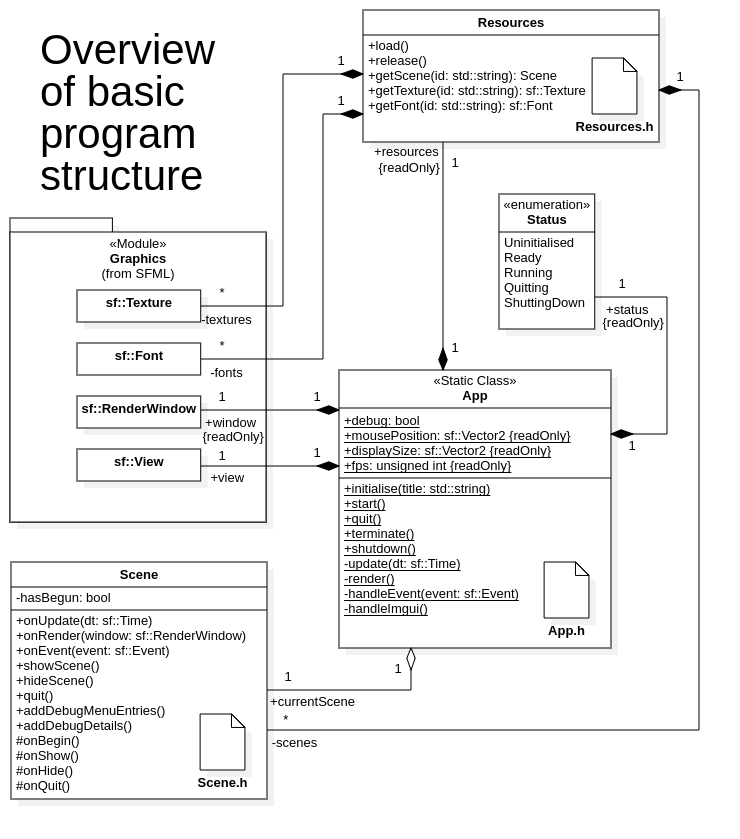
\includegraphics[width=\linewidth]{img/app_overview.png}
  \caption{A UML diagram detailing the infrastructure of the testing environment}
  \label{fig:foundationsUML}
\end{figure}

The first requirement listed in section \ref{subsec:requirements} is to create an interactive window that supports 2D graphics. Figure \ref{fig:foundationsUML} illustrates an overview of the program. The \emph{App} class manages the window and handles the main loop of processing input and rendering the screen. The \emph{Scene} class can be inherited to introduce different functionality to the testing environment and will be used to encompass the game and its logic. Since \emph{App} is entirely static, the game will have easy access to any of the application's variables or any data that has been loaded. \emph{Resources} acts as a manager and will store fonts, textures, scenes and eventually game-related data like maps. The enumeration \emph{Status} is used to determine what state the game is in --- the app is initialised with a title with \emph{initialise}, where it can then be given the first \emph{Scene} to use for when the game enters the main loop with \emph{start}. The \emph{start} function will then run continuously until the program is closed, starting the process of releasing resources before terminating the main loop closing the application.

\subsection{Designing the strategy game}
\label{subsec:designingStrategyGame}

The second requirement in section \ref{subsec:requirements} is to build a simple, turn-based strategy game for the AI to play. The rules of this game are simple: each player controls a squad of units with the aim being to eliminate all enemy units while maintaining at least one surviving unit. During their turn, a player can select one of their units and then move and attack with it. A player has a set amount of MP and AP (movement and action points) per turn, and can distribute them between each of their units. Each unit drains a different amount of MP per tile when moving and a different amount of AP when attacking as shown in table \ref{table:unitOverview}, meaning that some can move further and some can eliminate more units during a single turn. A unit can only attack another unit when it has enough AP and the target is in sight and range where nothing can be in between the attacker and their target.

\begin{table}[!h]
  \centering
  \begin{tabular}{ | l | p{6cm} | c | c | c |}
    \hline
    \textbf{Unit} & \textbf{Description} & \textbf{MP cost} & \textbf{AP cost} & \textbf{Range} \\ \hline
    Melee & Fast and close-range unit & 1 & 1 & 1 \\ \hline
    Blaster & Standard mid-range unit & 2 & 1 & 3 \\ \hline
    Sniper & Standard long-range unit & 2 & 2 & 10 \\ \hline
    Laser & Slowest unit with the longest range & 3 & 3 & 25 \\
    \hline
  \end{tabular}
  \caption{The traits each unit possesses in the game}
  \label{table:unitOverview}
\end{table}

Resource management and positioning are the two key elements that make this game strategic. A player will have to distribute MP between their units to keep them out of the enemy's range and line of sight while also positioning their units to attack the enemy safely. This won't always be possible; the constraints of the MP and AP mechanics mean that sacrifices have to be made each turn in order to win. This game will be suitable for answering the first and second research questions listed in section \ref{subsec:researchMethodologies} because moving and attacking can be directly linked to MP and AP costs allowing the A* algorithm to decide to move and attack units based on both positional and game-specific data.

Figure \ref{fig:strategyGameUML} shows the strategy game's structure and how the main \emph{Game} class is derived from the \emph{Scene} so that it can use functions such as \emph{update} and \emph{render} to integrate with the core program in section \ref{subsec:designingProgram}. The \emph{Game} class contains a lot of static functions such as \emph{readMap} and \emph{takeAction}, these functions are pure and do not rely on the current state of the game which is why they accept the data they operate on as a parameter rather than taking it from the instance of \emph{Game}. These functions are easier to reason about and can be safely used in any context without the state of \emph{Game} being touched --- this allows A* to make use of these functions to create, operate on and evaluate states of the game without making destructive changes.

\begin{figure}[!h]
  \centering
  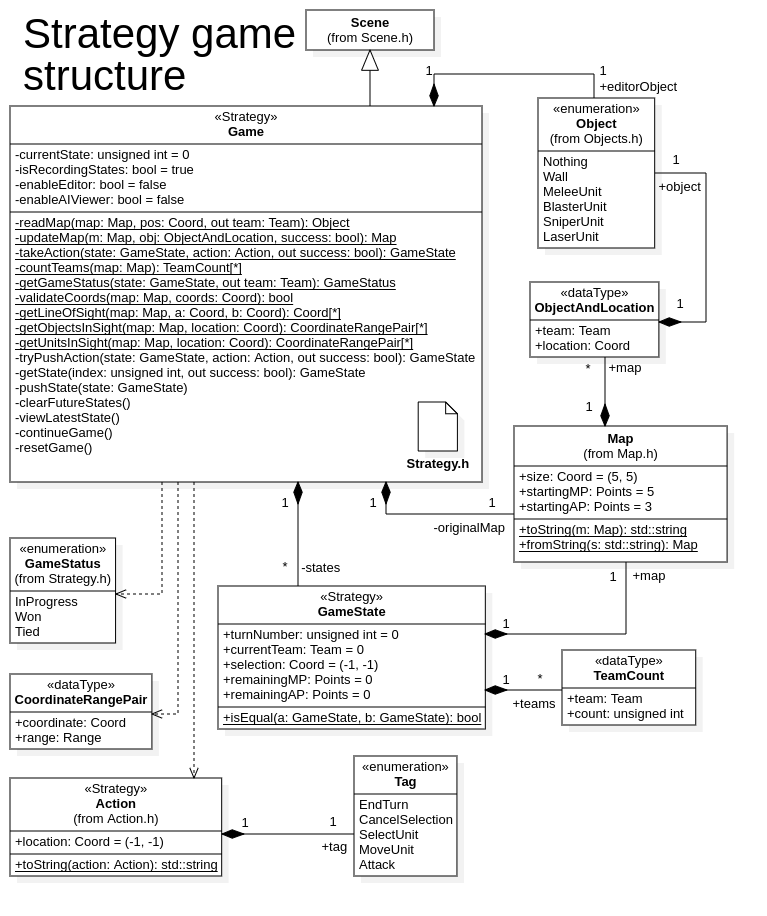
\includegraphics[width=\linewidth]{img/strategy_game_structure.png}
  \caption{A UML diagram showing the implementation of the strategy game}
  \label{fig:strategyGameUML}
\end{figure}

The actual state of the game is contained in the class \emph{GameState}. This is done for two reasons, the first reason being that these states can be collected and revisited as needed for the final requirement of section \ref{subsec:requirements}. The map, the currently playing team, the turn number and number of resources remaining are all contained within the \emph{GameState} itself and not in \emph{Game}; the game then uses the selected \emph{GameState's} contents to visualise the current state of the game on screen, making the viewing and overwriting of previous states as easy as viewing and manipulating this collection. The second reason is that the A* algorithm will process each \emph{GameState} as a node in the decision making process and the \emph{Actions} the players take will transform one state into a new, separate state to then be reconsidered for new \emph{Actions}. The \emph{GameState} class should represent what the AI's state and its perception of the game and be derived from the current state of the game, but because players have a complete set of information about the current state of the game, the \emph{GameState} class serves as both the AI's state as well as the actual state of the game.

\begin{figure}[!h]
  \centering
  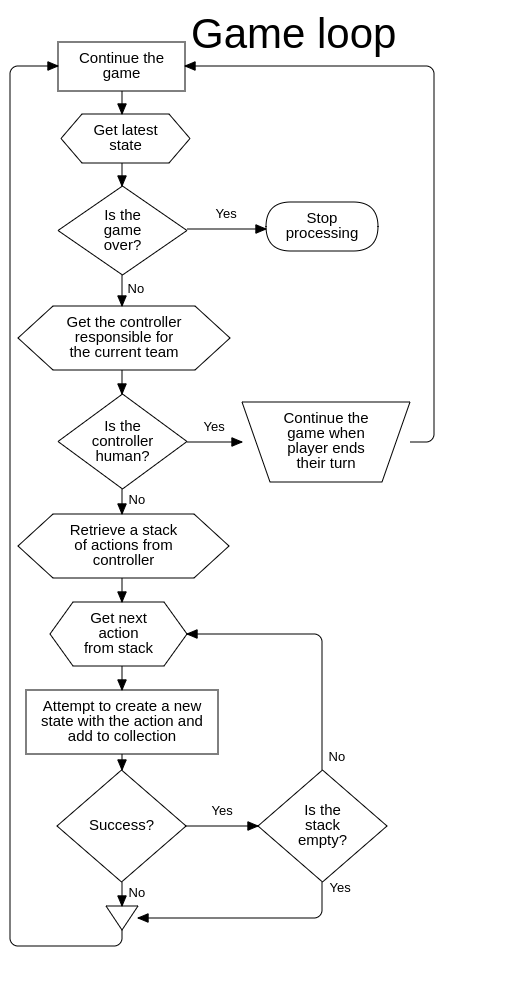
\includegraphics[width=12cm]{img/game_loop.png}
  \caption{A flowchart showing how a turn is executed}
  \label{fig:gameLoop}
\end{figure}

Figure \ref{fig:gameLoop} shows a flowchart of how a turn will be played out and will be introduced in the function \emph{continueGame} in the \emph{Game} class shown figure \ref{fig:strategyGameUML}. All controllers will return a stack of actions for the game loop to unwind and attempt to perform; this approach limits controllers to legitimate methods for working with \emph{GameStates} and that \emph{Game} can validate the decisions a controller makes and accept only those that are legal. The requirement of allowing a human to intervene section from section \ref{subsec:requirements} is also considered --- execution is will be interrupted during a human controller's turn and will resume when their turn ends. This process recursively fetches controllers' decisions and updates the collection of states until the game has concluded.

\subsection{Designing tools for debugging and observation}
\label{subsec:designingTools}

The requirements of a map editor and some way of browsing through the collection of states will be satisfied by using ImGui \parencite{Imgui} as stated in section \ref{subsec:toolAndFrameworkSelections}. Both the editor and state browser will be contained in their own windows so that the map editor can be hidden when not needed, however the state browser will always be on display because of how important it is for observation of the AIs.

\begin{figure}[!h]
  \centering
  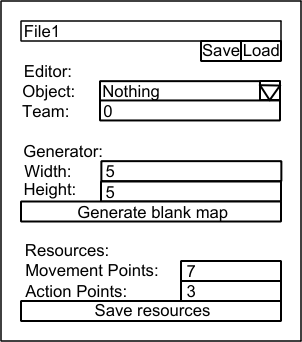
\includegraphics[width=10cm]{img/map_editor.png}
  \caption{A draft of the design for the map editor window}
  \label{fig:mapEditor}
\end{figure}

Figure \ref{fig:mapEditor} shows the four main parts to the map editor that are explained below:
\begin{itemize}
  \item \textbf{Saving and loading:} This can be implemented with a text input for entering the name of a file combined with two buttons for handling the saving and loading functionality respectively.
  \item \textbf{Creating and deleting objects:} As shown in figure \ref{fig:strategyGameUML}, an \emph{Object} is just an enum that can represent nothing, a wall or a unit. When paired with a \emph{Team} (represented as an integer value), a controller will then be assigned to that unit. This means that this part of the editor needs a drop-down box to select an \emph{Object} and a number entry for specifying the \emph{Team}. When the map editor window is open, left clicking and right clicking on the map will create and destroy objects.
  \item \textbf{Recreating maps:} This can be achieved with a number entries for specifying the width and height and a button that recreates the map when clicked.
  \item \textbf{Changing AP and MP:} Since changing the MP and AP requires the creation of a new \emph{GameState}, the only way to change these values is to push a duplicate of the current state with the new resources. This can be also be done after a new map has been generated before saving to set the MP and AP allocated per turn.
\end{itemize}

\begin{figure}[!h]
  \centering
  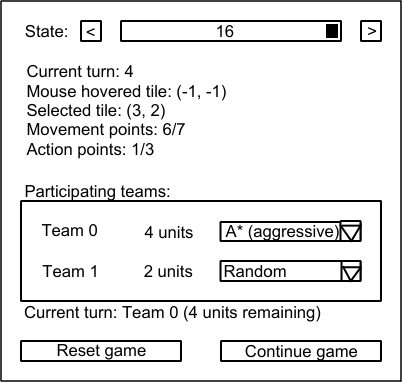
\includegraphics[width=10cm]{img/state_browser.png}
  \caption{A draft of the design for the state browser}
  \label{fig:stateBrowser}
\end{figure}

Figure \ref{fig:stateBrowser} shows how the state browser window should look. A simple scroll bar will suffice as a way of searching the collection --- the variable \emph{currentState} in \emph{Game} as shown in figure \ref{fig:strategyGameUML} is an index referring to which state in the collection \emph{states} to render on screen, so a scroll bar representing a range of values from zero to the size of \emph{states} creates an easy way of examine all states of the game. This window also displays information about the state, such as the amount of MP and AP as well as the number of members in each team. It makes sense to also include the ability to change the controller for each team since each team is already being displayed, this will allow the alteration of which algorithm is controlling which team at any given moment. Finally, the ability to reset and continue the game, clearing the state collection and starting the process illustrated in figure \ref{fig:gameLoop} respectively, will be introduced with the `reset game' and `continue game' buttons that can be seen at the bottom of the window.

Finally, a tool for viewing and adjusting details specific to every AI will be necessary for answering the third and fourth research questions from section \ref{subsec:researchMethodologies}. These questions require experimenting with different configurations when building game AI; since it is difficult to decide what these settings are without building the AI, having a flexible space for each AI to use would be beneficial. Introducing a state viewer would allow every AI to implement its own debugging functionality meaning that the tool will adapt to the AI and expose relevant variables for changing the AI without recompilation. Another use for an AI viewer would be to set up the same AI in different ways --- if an AI exposes variables, it may be interesting to make the AI play against itself with different settings. Since the point of the AI viewer is that it adapts to the AI that is currently playing, it will have no use with the other team controllers.

\pagebreak
\subsection{Designing the process of investigation}
\label{subsec:designingInvestigation process}

With the majority of the requirements in section \ref{subsec:requirements} designed, the only one unsatisfied is the actual implementation of the A* algorithm. A* will be programmed generically so that it can operate on various types. To function, A* requires a state type to act as the node, an action type to act as the edges and finally a cost type to represent the costs involved with traversing nodes --- the \emph{GameState} and \emph{Action} classes from figure \ref{fig:strategyGameUML} will be used for the nodes and edges, whereas the type of cost will be left up to each case so that different methods of representing cost can be tested.

\begin{table}[!h]
  \centering
  \hyphenpenalty=10000
  \begin{tabular}{ | m{2.5cm} | m{4cm} | m{6cm} |}
    \hline
    \textbf{Component} & \textbf{Description} & \textbf{Exemplary Changes} \\ \hline
    Goal function & Decide whether a given \emph{GameState} should be considered a goal & Making ending the turn or eliminating at least one enemy a goal to satisfy \\ \hline
    \emph{Cost} implementation & Represent and store the cost of performing an \emph{Action} & Separate the \emph{Cost} type into a set of different elements using various traits and aspects of \emph{Actions} \\ \hline
    Weighing function & Generate the suitable \emph{Cost} value for a given \emph{Action} & Changing how \emph{Actions} are valued to see how the AI's preferences affect behaviour \\ \hline
    \emph{Heuristic} function & Determine an order in which \emph{GameStates} are explored & Don't guide it (therefore using Dijkstra's algorithm) or try different ways of estimating the \emph{Cost} of satisfying the goal \\ \hline
    \emph{Cost} comparison function & Determine which \emph{Cost} is preferable to another & Experiment with multiplying and ignoring elements of \emph{Cost} as an alternative way of changing the AI's preferences \\
    \hline
  \end{tabular}
  \caption{The components of the A* algorithm and some examples of potential changes}
  \label{table:designingAStarVariations}
\end{table}

Since cases will implement their own \emph{Cost} class as well as the functions that operate on \emph{GameStates} and \emph{Actions}, each case will be implemented as a self-containing functor. These functors will exist in a collection in the \emph{Game} class and will be created and used when necessary. The functions in \emph{Game} shown in figure \ref{fig:strategyGameUML} will be common to all AIs, but functions such as the heuristic function are case-specific and will be member functions of each case's functor. Each case will use the A* algorithm differently with each variation being derived from interesting parts of the studies of previous iterations; if a flaw in one variation's approach is identified based on the behaviour observed, the next iteration might be adapted in an attempt to improve the current approach. The elements each variation could potentially change are listed in table \ref{table:designingAStarVariations}.

\section{Development}
\label{sec:development}

\subsection[Creating the application's foundations]{Milestone 1 --- Creating the application's foundations}
\label{subsec:creatingTheFoundations}

The first focus of development was to render 2D graphics, handle input, and to implement the \emph{Scene} class to allow for each self-containing sandbox to be integrated. Starting with \emph{main.cpp} and \emph{App.h}, there needed to be a way for the application to be set up and for the main loop to be started. Following figure \ref{fig:foundationsUML}, the main loop was implemented in the function \emph{start}, so \emph{initialise} needed to request for \emph{Resources} to \emph{load} everything in the asset directory. The \emph{initialise} function also opens the window and passes it to ImGui for rendering. ImGui comes with a demo feature, so the \emph{Console} class was also introduced so that debug messages can be displayed on-screen without needing a separate terminal.

Next was the \emph{start} function which keeps the application in a loop until it needs to close. From this loop, \emph{deltatime} will be calculated and given to \emph{update}, which doesn't do much other than store the location of the mouse cursor each frame for easy access. After \emph{update}, any input detected by SFML gets polled and passed to the \emph{handleEvent} function where it is decided which class should receive the event --- if the user has clicked on an ImGui window, all text input should be given to ImGui so that they don't accidentally interact with games in the application. Finally, the \emph{render} function is called which is responsible for clearing the screen, telling ImGui to render, and displaying that has been drawn onto the screen. A master debug menu will be displayed when \emph{App}'s debug flag is set to $true$. This menu will show various, generic information about the application such as the frames per second and the cursor location. Additionally, it is through this menu that \emph{Scenes} can be swapped to and their scene-specific debug windows can be shown and hidden.

\begin{figure}[!h]
  \centering
  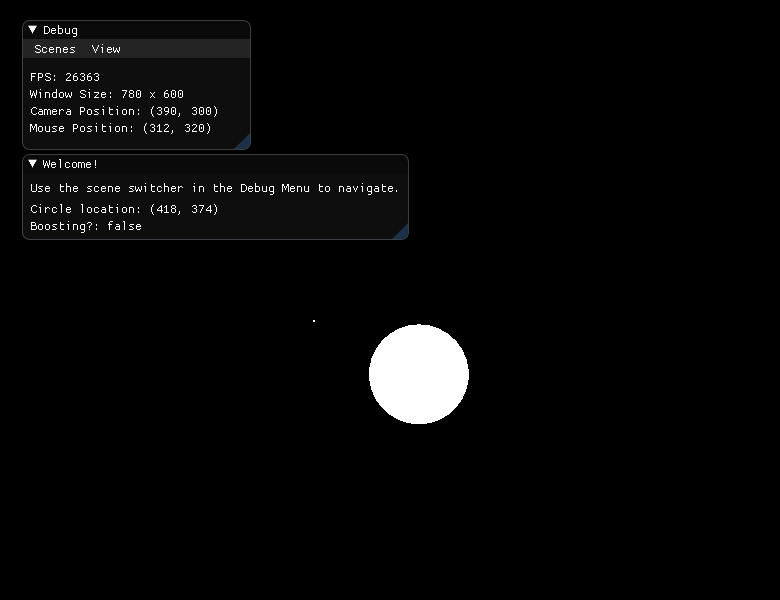
\includegraphics[width=\linewidth]{img/welcome_scene.png}
  \caption{A screenshot of the welcome scene}
  \label{fig:welcomeScene}
\end{figure}

After the application successfully looped, all that was needed was to implement the \emph{Scene} class and to call functions \emph{showScene}, \emph{hideScene}, \emph{onUpdate}, \emph{onEvent} and \emph{onRender} on \emph{App}'s current \emph{Scene} from their \emph{App} counterparts. The function \emph{switchScene} is introduced to \emph{App} so that the beginning, showing and hiding of \emph{Scenes} can be done automatically; this function accepts a string and will query \emph{Resources} for a pointer to the relevant \emph{Scene}. \emph{Scenes} can also implement \emph{addDebugMenuEntries} and \emph{addDebugDetails} to add functionality to the debugging interface mentioned above. In order to test that the \emph{App} can be started, switched to a \emph{Scene}, and interacted with, the welcome \emph{Scene} shown in figure \ref{fig:welcomeScene} was made which featured a white circle that followed a mouse and an ImGui window specific to the \emph{Scene}.

\subsection[Building a sample game]{Milestone 2 --- Building a sample game}
\label{subsec:buildingASampleGame}

Before the A* algorithm can be implemented for experimentation, there needs to be something in place for it to operate on and process. Since this project is being developed in an agile way, it was decided that a small, well-known and easily programmable game would be used to get a greater understanding of the requirements for this approach to game AI in case they need to be changed later. Tic-tac-toe fit this criteria well and served as a way of gauging the plausibility of creating game AI using A*. This game would also make use of a controller class so that trivial AI, complex AI, and humans can play the game, allowing the implementation of A* to easily be tested against a human as it was being built. The human controller was created first so that the rules of tic-tac-toe could be tested before an AI was introduced. The random team controller mentioned in section \ref{subsec:requirements} came next: it chooses randomly from all available actions until it's turn is over. The idle controller cannot be implemented for tic-tac-toe as turns cannot be skipped.

\begin{figure}[!h]
  \centering
  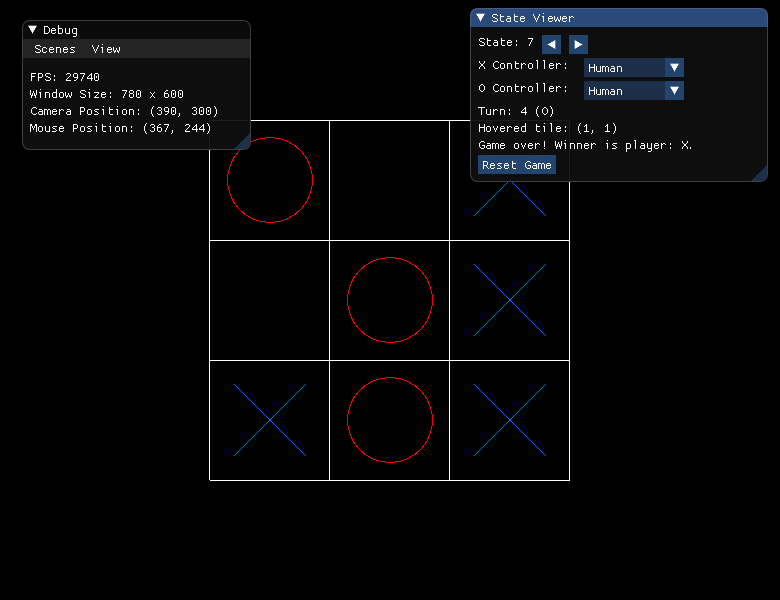
\includegraphics[width=\linewidth]{img/tictactoe_game.png}
  \caption{A screenshot of the tic-tac-toe game}
  \label{fig:ticTacToeGame}
\end{figure}

It is logical to build the tic-tac-toe game in the same way as the final game so that designs and implementations can be tested early, and so the tic-tac-toe game will make use of a \emph{GameState} class so that turns can be undone and replayed. A simplified \emph{GameState} viewer has been created with ImGui so that it can be tested as well --- if appropriate, parts of this tool would be reused later to save time when developing the final version of the game. Figure \ref{fig:ticTacToeGame} shows the tic-tac-toe game with fully functioning human controllers and \emph{GameState} viewer.

\subsection[Implementing and allowing A* to play a game]{Milestone 3 --- Implementing and allowing A* to play a game}
\label{subsec:implementingAndAllowingAStarToPlay}

With the simple game built in section \ref{subsec:buildingASampleGame}, it was time to re-engineer the A* algorithm to operate on non-spatial data and play tic-tac-toe. This generic implementation of A* is shown in appendix \ref{appendix:genericAStarImplementation} --- the algorithm remains the same as the standard A* with a one exception: the types of the nodes, edges and the costs they evaluate to were replaced with the C++ templates \emph{S}, \emph{A} and \emph{C} respectively. Doing this meant that the algorithm had further requirements, as there was no longer any way to calculate the distance between two instances of \emph{S}, or any way of expanding nodes. Function pointers, or alternatively a functor could be used, solve this by requiring this functionality being passed in when the algorithm is used. For instance, if used for pathfinding, this algorithm would be given a function that would find adjacent tiles or waypoints to a given node so that nodes can be expanded properly. The types and functions supplied for the AI to play tic-tac-toe are listed below:

\begin{itemize}
  \item \textbf{States:} The states of the game are represented by the tic-tac-toe \emph{GameState} class.
  \item \textbf{Actions:} A move is made by placing a mark in the grid, so an action is just a location represented by a pair of integers (the \emph{sf::Vector2i} class).
  \item \textbf{Costs:} An integer value represents the penalties for making illogical moves.
  \item \textbf{Goal node identification:} Every action was valid as long as a mark was placed on an empty space, therefore the AI wasn't directed towards a specific goal but rather to just make a move. Since comparing the current node and the starting node might become a common occurrence, the implementation of A* was adjusted so that the \emph{isStateEndpoint} function accepts both of these nodes, meaning that these states can be easily compared when checking to see if a given state should be considered a goal.
  \item \textbf{Node expansion:} Took a \emph{GameState} and finds empty spaces for marks to go to return a collection of actions and the \emph{GameStates} they led to.
  \item \textbf{Cost comparison:} Costs were represented as an integer, so finding the lesser value was trivial and the standard $<$ operator was used.
  \item \textbf{Heuristic function:} No heuristic was supplied --- $h(n)$ returned the same value and therefore A* turned into Dijkstra's algorithm for this test.
  \item \textbf{Weighing function:} Penalties were applied in accordance to how inappropriate a move was. Moves which didn't finish possible game-winning rows of three are heavily penalised to ensure that the AI would win when it can. Similarly, moves which didn't block two marks in a row owned by the opponent were severely penalised to incentivise blocking the opponent's obvious attempts of winning. Other than that, the penalty of a move would depend on how many `near-wins' are created for the AI and how many are left unchecked by the opponent. This is an arbitrary function and will be scrutinised during the actual experiment.
\end{itemize}

While the AI did play the game successfully, it didn't prove whether game AI using A* was actually plausible. Each turn in a game of tic-tac-toe consists of exactly one move, and so the A* algorithm was creating a sequence containing a single action --- it compared all possible moves and chose the option that was penalised the least by the weighing function. From this, more requirements for the experiment could be identified; a game where the AI can do multiple actions per turn would provide results with greater detail and would be a more realistic use case. The requirements in section \ref{subsec:requirements} and the design of the game in section \ref{subsec:designingStrategyGame} were changed to reflect this realisation. Additionally, since this game is going to feature a lot more states than tic-tac-toe and the only way of revisiting previous states was to click the arrow buttons shown in figure \ref{fig:ticTacToeGame}, the design of the state viewer in section \ref{subsec:designingTools} was changed to include a scrollbar for faster browsing of states.

\subsection[Building the final game]{Milestone 4 --- Building the final game}
\label{subsec:buildingTheFinalGame}

After programming and testing the A* algorithm, the final piece before the case studies could be started was the game itself. The game designed in section \ref{subsec:designingStrategyGame} was built from the ground up to support both human and non-human players; visuals on the screen ensured that information such as sight lines and the resources remaining was properly communicated regardless of state. Units were represented by letters and their colour shows which team they are on. Additionally, the generic implementation of A* was used for standard pathfinding, so that players didn't have to move their units step by step. Figure \ref{fig:strategyGame} shows the finished game in action from a human player's perspective, showcasing the pathfinding of the melee unit in conjunction with the resource cost for performing the manoeuvre.

\begin{figure}[!h]
  \centering
  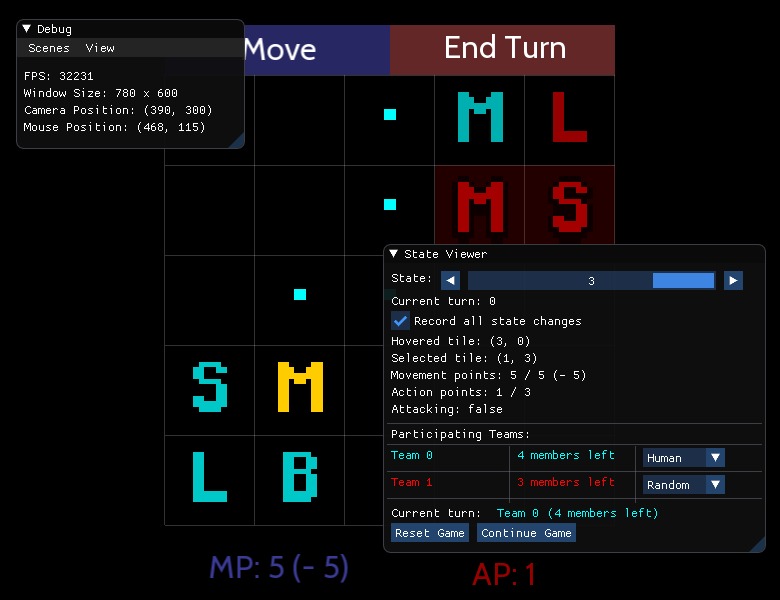
\includegraphics[width=\linewidth]{img/strategy_game.png}
  \caption{A screenshot of the strategy game showing a turn in progress}
  \label{fig:strategyGame}
\end{figure}

The state viewer and information window created in section \ref{subsec:buildingASampleGame} was adjusted to show details about the new game, as well as being expanded to handle multiple teams playing a single game. Finally, the map editor as well as the ability to save and load maps were introduced. Overall, development went smoothly --- having the tic-tac-toe and strategy games share similar approaches using \emph{GameStates} and a variety of static functions meant that development was a matter of adapting and expanding previously written functions to suit the new game. With the human and trivial controllers properly set up to play the game, the case study could finally begin.

\section{Results and Evaluation}
\label{sec:resultsAndEvaluation}

\subsection{Case study one}
\label{subsec:caseStudyOne}

\subsubsection{Configuration}

\begin{itemize}
  \item \textbf{Goal:} A \emph{GameState} is considered a goal node when the currently playing team changes, meaning that the previous \emph{Action} was the ending of the current turn and give control to the next team.
  \item \textbf{Cost:} Represented by a set of integer values representing different penalties: enemies remaining, allies lost and allies at risk. The aim is to make the AI select actions that eliminate opposing units without exposing allies. Friendly fire is also an option and actions that kill an allied unit are given penalties. Summing \emph{Cost} values is achieved by adding the components together, resulting in a \emph{Cost} value containing totals for each penalty.
  \item \textbf{Cost comparison:} A \emph{Personality} class has been introduced which contains floating point values as multipliers for the elements of \emph{Cost}. When comparing two \emph{Cost} instances, their values are manipulated by a \emph{Personality} before being summed into one value, it is these totals that are then used in comparisons.
  \item \textbf{Heuristic function:} Nothing useful given --- only a \emph{Cost} value containing zero for each penalty is given.
  \item \textbf{Weighing function:} Shown in appendix \ref{subsec:caseOneWeighingFunction}, each element of \emph{Cost} is found through comparison of \emph{GameStates}. Constant arbitrary values are used to create the penalties; for example, 10 points are added to the `enemies remaining' penalty total. Selecting units or ending the turn doesn't change the map and aren't penalised.
\end{itemize}

This approach is very similar to the way the AI in tic-tac-toe compared different moves. No goal or heuristic was provided, so the AI relied entirely on the \emph{Costs} generated by the weighing function shown in appendix \ref{subsec:caseOneWeighingFunction}. The notion of a \emph{Personality} was introduced to tweak the AI's values; perhaps it is desired for the AI to not care about killing friendly units if it means winning. Ending the turn doesn't award any penalties because the \emph{Cost} of the \emph{Action} sequence comes from what the AI does, and since ending the turn does nothing to the game there's no reason to add a penalty for it.

\subsubsection{Observations}

The AI displayed no behaviour regardless of which map from appendix \ref{appendix:strategyGameMaps} was selected, although it still managed to win due to the random controller killing its own units. It instantly ended its turn like the idle controller. This reinforces how poor tic-tac-toe was for experimentation; the lack of depth meant that this flaw remained unexposed. As discussed in \ref{subsec:definingTheNotionOfCost}, A* uses non-negative cost values so that higher-costed action sequences can be deferred. With every move being penalised on some scale, performing two \emph{Actions} in a row will typically cost more than performing a single \emph{Action} even if the resulting \emph{GameState} is more favourable. Since there wasn't a non-zero \emph{Cost} for ending the turn, there wasn't a combination of \emph{Actions} that was preferable to doing nothing.

This case illustrates one flaw of developing game AI in this way: there must be extra consideration for possibly numerous areas of the AI in order to ensure that the behaviour is within expected parameters. Further cases need some way of deferring the ending of the turn.

\subsection{Case study two}
\label{subsec:caseStudyTwo}

\subsubsection{Configuration}

\begin{itemize}
  \item \textbf{Goal:} End the current turn.
  \item \textbf{Cost:} A collection of integer values as described in case study one, but with additional penalties for wasting MP and AP.
  \item \textbf{Cost comparison:} Same method of comparison as case study one.
  \item \textbf{Heuristic function:} Nothing useful given --- only a \emph{Cost} value containing zero for each penalty is given.
  \item \textbf{Weighing function:} Shown in appendix \ref{subsec:caseTwoWeighingFunction}. The end turn \emph{Action} applies a heavy penalty based on how much MP and AP is remaining.
\end{itemize}

This case is almost identical to case study one from section \ref{subsec:caseStudyOne}; in that case study, the AI chose to do nothing every time because the end turn \emph{Action} was weighed to have zero \emph{Cost}. As shown in appendix \ref{subsec:caseTwoWeighingFunction}, ending the turn now incurs a penalty depending on how much MP and AP is remaining in an attempt to incentivise performing \emph{Actions} and spending these resources to lower the penalty. One final thing that was considered was the multiplying of all elements of the \emph{Cost} value when the turn is ended. This is so that additive and multiplicative penalties can be tested in case one is more effective than the other. The AI viewer will allow the manipulation of these values so that different behaviours can be found during play.

\subsubsection{Observations}

Initially, when playing on the map \ref{sec:mapDefault5x5} the AI didn't move at all and repeated the behaviour of case study one in section \ref{subsec:caseStudyOne}. After manipulating the multiplier for MP and AP penalties, the AI was quickly compelled to win the game against both the idle and random team controllers. This is because the penalty for wasting MP and AP becomes great enough that ending a turn with less resources and killing more enemies is favourable to doing nothing, which is promising. It doesn't matter how high these penalties were set; when the same amount of resources have been spent, the AI will take the other penalties into consideration to find the absolute minimum. One humorous event that occurred was when the AI played against itself: because the second case's AI greatly valued spending resources, it actually eliminated itself when there was only one unit of its squad left after being wiped them out in the first turn. Figure \ref{fig:caseStudyTwoSuicide} shows this AI in action as well as this comedic moment.

\begin{figure}[!h]
  \centering
  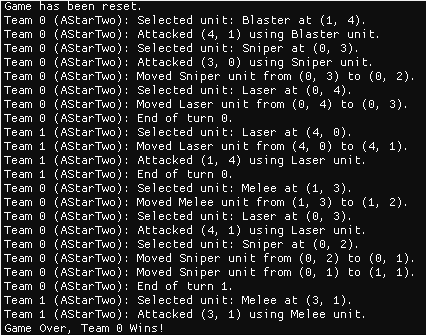
\includegraphics[width=12cm]{img/case_two_suicide.png}
  \caption{Log of the game where case study two played against itself}
  \label{fig:caseStudyTwoSuicide}
\end{figure}

Increasing the total turn multiplier from one slowed down the turn dramatically, becoming impractical at multipliers higher than 3. It is suspected that this is because A* cannot terminate computation until it reaches a goal node or it runs out of open nodes, and doing this postpones the evaluation of all end turn \emph{Actions} until every other \emph{Action} has been processed. This is unhelpful and inefficient.

This AI heavily struggled with map \ref{sec:mapCrossWall5x5}. The AI took a lot longer to win the game in real time, taking almost 10 minutes with the MP and AP multipliers set to 5 and the end turn multiplier set to 1. This demonstrates another flaw in using penalties to influence AI --- A* was constantly evaluating nodes with the lowest \emph{Cost}, and so because there was no way of ending the current turn without incurring a large penalty, the algorithm had to process the majority of possibilities before an end turn \emph{Action} would be considered the next thing to process. Multiple sets of values were tested, but a solution to speeding up the AI could not be found. Further cases will need to consider the following:

\begin{itemize}
  \item Using a heuristic function to perform best-first searches, which could be difficult because `best' is subjective when it comes to gameplay.
  \item Limiting the depth of the search, although there needs to be some sort of backup in place.
  \item Changing penalties in some way so that the AI isn't penalised for performing \emph{Actions} in a bad situation.
\end{itemize}

\subsection{Case study three}
\label{subsec:caseStudyThree}

\subsubsection{Configuration}

\begin{itemize}
  \item \textbf{Goal:} End the current turn.
  \item \textbf{Cost:} A single integer value that increases based on the penalties applied.
  \item \textbf{Cost comparison:} Standard integer comparison using $<$ operator.
  \item \textbf{Heuristic function:} No useful heuristic given.
  \item \textbf{Weighing function:} New implementation as shown in appendix \ref{subsec:caseThreeWeighingFunction}. The new function is long and cluttered, but avoids applying penalties to any \emph{Action} that could be considered a good move. The body of the function is split between every type of \emph{Action} and will only penalise if the resulting \emph{GameState} is worse than the previous. The \emph{Action} for unit selection has a fixed to stop infinite loops since selecting units does not do anything destructive to the \emph{GameState}.
\end{itemize}

Following from case study two in section \ref{subsec:caseStudyTwo}, this case is only interested in changing the approach to assigning \emph{Costs} to \emph{Actions}. The previous cases have challenged the AI to choose the least penalised option, but this caused complications in situations where no sequence of \emph{Actions} could be seen as an objectively good move from the AI's perspective. Now, a large amount of \emph{Actions} can have zero \emph{Cost}. Only the \emph{Actions} that aren't effective are penalised; moving units out of sight or range and eliminating units are examples of \emph{Actions} that are potentially free depending on the situation. One final thing to note is that this weighing function has a goal embedded into, where survival is only prioritised when on a low unit number, and eliminating the enemy is the standard objective --- this is so that the AI is encouraged to fight rather than hiding in a corner, which could otherwise be considered the better move. This embedded goal could be factored out later when experimenting with goal nodes. When ending the turn, the \emph{GameState} is compared to the starting state and penalties are applied for the amount of enemies left alive.

The AI will use these zero-cost edges to identify all possible end points. It will then expand any non-free edges that have an $f(n)$ lower than the lowest-costing end point. Unless anything else is found, the sequence that leads to the end point with the fewest penalties is chosen. This algorithm may be slow if there's a large number of free options, which is why a thorough weighing function is required to ensure that a large portion of \emph{Actions} are non-free. This will effectively give us something similar to what happened in case study two, where the evaluation of the end-turn \emph{Actions} happen later on, but this time the pool of nodes to be expanded should be smaller and therefore the AI should be able to handle more situations.

\subsubsection{Observations}

The AI won swiftly and intelligently on maps \ref{sec:mapDefault5x5} and \ref{sec:mapCrossWall5x5} against the idle and random controllers. Figure \ref{fig:caseStudyThreeGame} shows how differently this AI plays on map \ref{sec:mapDefault5x5} when compared to case study two in figure \ref{fig:caseStudyTwoSuicide}. In this case, team 0 eliminated three members of the opposing squad quicker than case study two and also tries to retaliate when losing.

\begin{figure}[!h]
  \centering
  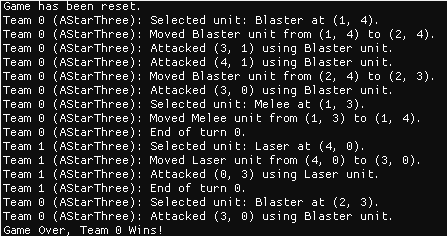
\includegraphics[width=12cm]{img/case_three_game.png}
  \caption{Log of the game between case study three played against itself}
  \label{fig:caseStudyThreeGame}
\end{figure}

This AI is very promising, but there isn't enough space to create maps that produce interesting gameplay when limited to 5x5. Moreover, without testing for the limits of each AI, it is difficult to answer the research question from section \ref{subsec:researchMethodologies}: "how plausible is it to use A* in a decision making process for game AI?" With this, it has been decided that the preferred map size should be 7x7 so that a greater variety of behaviour can be observed. Map \ref{sec:mapDefault7x7} has been creating as the new default map. Unlike the previous AIs, this AI can handle a map this large although there is a noticeable reduction of speed.

After two minutes in real time, this AI processed over 1500 possible \emph{GameStates} with 2000 unexplored before taking its turn on map \ref{sec:mapDefault7x7}. Since eliminations were made, the subsequent turns were processed almost instantaneously when playing against any of the controllers so far. On its first turn, the AI made use of the blaster and laser units. It chose the high-cost laser unit over the sniper unit to ensure that it used up all of its resources; both units have the same effective range as shown in table \ref{table:unitOverview}, but with the squads being far apart from each other no other unit could have attacked and so the AI would have wasted at least 1 AP. Figure \ref{fig:caseStudyThree7x7Game} demonstrates this: the human controller shows visualisations of the range and sight of units when attacking, from this it can be calculated that the blaster and sniper units could not have made two eliminations, and so the AI found the one unit that could make the attack.

\begin{figure}[!h]
  \centering
  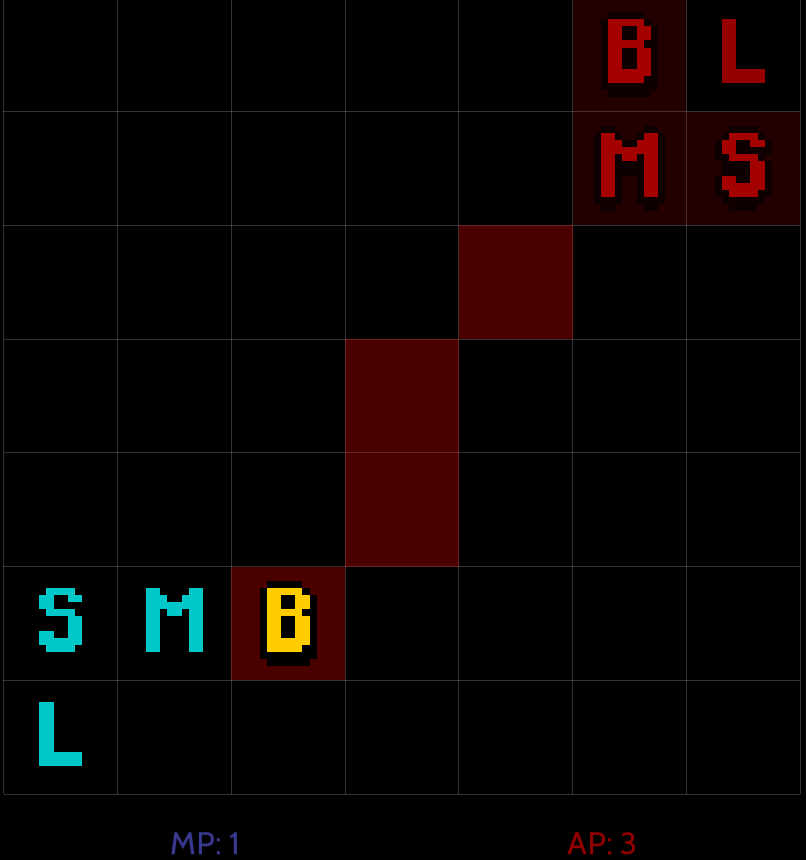
\includegraphics[width=10cm]{img/case_three_7x7_game.png}
  \caption{Screenshot showing how the blaster unit could not have attacked in turn one}
  \label{fig:caseStudyThree7x7Game}
\end{figure}

This shows that this AI can be intelligent by choosing the lowest costing route. Applying a heuristic function could make this process faster, as even though the AI plays well on both map \ref{sec:mapDefault7x7} and map \ref{sec:mapCrossWithBlock7x7}, it has to process thousands of states before making a decision. In particular, over 5000 states were in the open list on the second turn of map \ref{sec:mapCrossWithBlock7x7} against an idle controller --- this is expensive in terms of both speed and memory consumption. Game AI doesn't always have to make the best decision, so further case studies should attempt to reduce the number of states processed while preserving an acceptable amount of intelligence.

\subsection{Case study four}
\label{subsec:caseStudyFour}

\subsubsection{Configuration}

\begin{itemize}
  \item \textbf{Goal:} Eliminate a unit or move closer to the enemy. This goal can be toggled on or off using the AI viewer. Shown in appendix \ref{subsec:caseFourGoalFunction}.
  \item \textbf{Cost:} A single integer value that increases based on the penalties applied.
  \item \textbf{Cost comparison:} Standard integer comparison using $<$ operator.
  \item \textbf{Heuristic function:} New implementation (\ref{subsec:caseFourHeuristicFunction}). The heuristic attempts to predict upcoming penalties. Separate from penalties, prediction values are a rough estimate of the penalties the AI will take when meeting the prediction. Every enemy that is alive and every ally that needs to be hidden behind cover contributes to the heuristic cost using these prediction values. When the goal is enabled, the distance to the closest enemy will also be factored in if an enemy hasn't been eliminated.
  \item \textbf{Weighing function:} New implementation (\ref{subsec:caseFourWeighingFunction}). Lightweight function that only penalises unproductive \emph{Actions} such as attacking allied units or nothing at all. There are various optional penalties to manipulate, such as cost per resource spent, the cost of performing any \emph{Action} and the cost of ending the turn.
\end{itemize}

This case aims to improve case study three in section \ref{subsec:caseStudyThree} through the introduction of heuristics. As discussed in section \ref{subsec:aStarAlgorithm}, the heuristic function allows A* to be balance of speed and accuracy; this case aims to replicate the intelligence of case three while being more capable of processing the 7x7 maps such as \ref{sec:mapDefault7x7} and \ref{sec:mapCrossWithBlock7x7}.

A* uses the fitness of a node, $f(n)$, to determine whether it should be explored next. So far, only the real cost of navigating to that node, $g(n)$, has been investigated through the weighing function. The effectiveness of A* relies on \emph{Costs} being non-negative and never losing value, so $g(n)$ of a node shouldn't decrease. When using A* for game AI, the \emph{Actions} performed later can never make up for \emph{Costs} incurred by the \emph{Actions} done previously in a sequence. This is where heuristics are helpful, as $h(n)$ can decrease and potentially lower $f(n)$ as a result. In standard pathfinding, the heuristic distance decreases as the goal node is approached; this is reinterpreted in this case's heuristic function. The previous cases preferred nodes that had a lower cost to perform, whereas this case prefers a node because it improves the fitness of the sequence in some way.

The notion of a goal has also been introduced in an attempt to influence the AI towards engaging enemy units. Case study three worked very well with its elaborate weighing function, but its goal was hard-coded into the weighing function so that it preferred \emph{Actions} that resulted in conflict. This case uses the \emph{isEndPoint} function to restrict which nodes are considered goals. This isn't a trivial function to implement --- the goal must always be achievable, otherwise the algorithm will finish execution with a failed result and, in the case of this game, nothing will happen. If the goal was to kill an enemy unit each turn, the AI would be unable to act in situations where attacking is impossible, such as if the enemy was too far away. The goal node is not what is expected; it is what is required. That is why the goal for this case was to kill an enemy unit \emph{or} move closer. \emph{Actions} that end the current turn are considered dead-ends instead of goals if they haven't fulfilled the requirements of the goal. The heuristic function can also take this goal into account. At first, nodes are generally unfit, but moving towards the enemy is an easy way to lower and improve $f(n)$. Eliminating an enemy unit removes this component of the heuristic entirely to further incentivise the AI to attack when possible.

With the heuristic function playing the largest role, the role of the weighing function is to value an \emph{Action} based on what is sacrificed permanently. Shooting allies and ending the turn are both examples of choices with consequences. Shooting an ally reduces the fitness of the rest of the sequence, which is what $g(n)$ should truly represent. The only reason for the algorithm to explore a node with a higher $g(n)$ will be if $h(n)$ is low enough to compensate, the aim being to give the AI the ability to make sacrifices. This case also investigates the idea of resource investment: there is an optional penalty for using the MP and AP spent in the weighing of an \emph{Action}. These penalties are also applied when the turn is over so that the AI can decide between spending resources to end the turn and spending them to perform more \emph{Actions}. Hopefully, a result similar to that of case three's usage of free \emph{Actions} will be found without needing to make everything free.

\subsubsection{Observations}

The AI shows a wide variety of behaviour, from total inactivity to winning the game, depending on the values for penalties provided. The algorithm also finished execution much faster than case study three in section \ref{subsec:caseStudyThree}, and was much easier to test on the default 7x7 map in appendix \ref{sec:mapDefault7x7}. Below is a list of notable tests involving case four:

\begin{description}

\item[Map \ref{sec:mapDefault5x5} against case study three:] Case three won regardless of which team went first. Case three has a more elaborate weighing function and can tell the difference between a good and bad \emph{Action} better. After processing a large amount of possibilities, it chooses the best one, and so in most situations it will win. Case four doesn't evaluate a lot of states because of the heuristic, allowing it to make decisions much faster. Unfortunately, regardless of the amount of combinations of attempted, it was difficult to make case four a stronger AI. It played the game and served well as an opponent, but on this map it is relatively easy to eliminate three units in a single turn; case four doesn't attempt to eliminate more than one.

\item[Map \ref{sec:mapCrossWall5x5} against itself:] All of the AIs so far have struggled with maps with walls. Unfortunately, so did this one, taking a couple of minutes to process approximately 1500 nodes. While it didn't take as long to generate a solution as the previous AIs, it still took an impractical amount of time. The AI chose to destroy the center block and attack diagonally to minimise the amount of blocks destroyed, rather than creating more space. This was probably the smartest decision, as the team that destroys the walls waste their AP just to expose themselves to the enemy.

\item[Map \ref{sec:mapDefault7x7} against itself:] Towards the end of the game, the AI ended its turn early. When the \emph{GameState} was revisited and the AI was restarted, it made the decision to attack and eliminate the remaining unit and win the game rather than spare them like it did before. After adjusting the values for each penalty, it appeared that using MP and AP to weigh edges wasn't important to the process but was in fact detrimental. After setting the cost of spending MP and AP to 0, these kinds of judgements stopped occurring. The previous tests were re-ran to ensure with the new numbers in case anything changed but nothing was noticeably different.

\item[Map \ref{sec:mapDefault7x7} against study three:] In contrast to when playing on map \ref{sec:mapDefault5x5}, case four won against case three when going first. On the 5x5 map, it was illogical to not eliminate the majority of the enemy squad which is why it lost. On this map however, eliminating the enemies one by one sufficed to win the game. This was still unexpected, as case three has proven to be highly capable when given enough time to process, and it was expected that would calculate a counter attack --- not doing so suggests that such a tactic was not an option. This result suggests that case three doesn't excel at every type of problem when not in control, and that even when given control, case four isn't guaranteed to be intelligent.

\item[Map \ref{sec:mapCrossWithBlock7x7} against anything:] Unfortunately, none of the AIs managed to play on this map without requiring a large amount of time.

\end{description}

Case four's AI was very difficult to experiment with. Without embedded behaviour like case three, it entirely relied on the value and relationships between penalties. Trying to make the AI prioritise eliminating enemy units instead of ending the turn was frustrating as trial and error is the only way to determine which combination of values do what. The higher the value of a penalty, the higher priority it will be to be avoided. This appeared to be useful in the beginning, but unlike state machines or behaviour trees there is no easy way of knowing why the AI chooses to do what it does. When trying to make case four's AI stronger, it was difficult to determine which penalties translated to gameplay strength. The easiest way of making a stronger AI would be to expand the heuristic and weighing functions to be more like the one in case three, but that would make it less flexible.

\subsection{Summary}
\label{subsec:summaryOfCaseStudies}

The investigation has reached its conclusion. While it would be possible to create any number of AIs, it is believed that the research questions posed in section \ref{subsec:researchMethodologies} can be answered from the pool of AIs that have been created. Further AIs would have been created if the results had been more positive, but at this stage the creation of further AIs would simply provide more examples of problems already identified and not yield anything of benefit. Recall from section \ref{subsec:makingDecisionsWithAStarUsingGOAP} that these AIs are not the only examples of using A* for decision making and that GOAP \parencite{orkin2003applying} was used for the AI in the game F.E.A.R \parencite{FEAR}. There are significant differences between the approaches used in this investigation and GOAP; they are only related in the sense that they both use the A* algorithm, but there are clear distinctions between the implementations, usages and behaviours of their resulting AIs.

\subsubsection{How plausible is it to use A* in a decision making process for game AI?}

The existence of GOAP already demonstrates that A* can be used for AI purposes. However, the case studies suggest that A* is rather unsuitable for AI. Case study one in section \ref{subsec:caseStudyOne} demonstrates the most common flaw of reimplementing a search algorithm for AI: the AI has a tendency to do nothing unless it is told that doing nothing is wrong. This is problematic, as it should be valid for an AI to do nothing in the correct situation. This problem appeared in the creation of all case studies and the requirement for overcoming it introduces awkward and arbitrary elements to the AI. Telling the AI what not to do, as opposed to what it should do, makes both creating and changing behaviour difficult.

Another flaw in creating AI in this way is that it is hard to be certain about how the AI's programming will affect behaviour. Every subsequent case study used different weighing functions, each having valid and constructive reasoning. However, in spite of the effort placed into designing these functions it can be concluded that the behaviour of each AI varies drastically and cannot be predicted from the programming alone. This aspect is likely unappealing to game developers, as there's no way of knowing how the AI will behave or whether it is going to break in a given situation. With these things considered, the approaches created in this investigation have not produced any results showing signs of suitability and GOAP continues to be the most successful approach for applying A* to game AI.

\subsubsection{How does the inclusion of pathfinding affect decision making?}

GOAP's \emph{Actions} are used differently when compared to the \emph{Actions} in this game: GOAP's \emph{Actions} are simple and only one instance is created for each type of \emph{Action}, whereas in this investigation an \emph{Action} instance was created for every opportunity so that they could integrate with the pathfinding process instead of replacing it. Where GOAP's AI would perform a single \emph{Move Action}, the AIs observed in this study would have to perform a \emph{Move Action} for moving to each tile when pathfinding. For GOAP, the choice to attack comes purely from the \emph{Attack Action}, whereas in this study the AIs evaluated each possible \emph{Attack} from each possible location. GOAP's locations and targets are chosen based on the goals provided which reduces the number of \emph{Actions} and \emph{States}. In this study, the selections were made within the decision making process which had the opposite affect and inflated these numbers, having consequences in the performance and behaviour of A*.

Case three in section \ref{subsec:caseStudyThree} displayed promise for eliminating enemy teams intelligently. The AI had great gameplay strength and achieved a high aptitude for finding the best outcome of a situation. Feeding all possible situations to A* allows it to find the best sequence of \emph{Actions}; when a heuristic is provided such as in case four in section \ref{subsec:caseStudyFour}, the algorithm has the ability to terminate early with an acceptable solution that isn't necessarily the best. Cases three and four demonstrate that A* can make decisions such as where to move and who to attack when given a large number of options, but they also reveal the resulting impact on performance that makes these AIs unsuitable for more realistic applications. In normal pathfinding on a grid, an agent using A* can move in four directions and the number of routes becomes manageable, but the AIs in this investigation can also attack, select a new unit and end their turn. This means that instead of 4 edges per node A* has to process roughly 10--20, greatly increasing the total number of nodes and the time to process a suitable sequence of \emph{Actions}. Replacing the game with one that features less interactions would benefit the AI, but the game used in this experiment could already be considered a simplification when compared to commercial games and simplifying things further would not provide any insights applicable to most use cases.

\subsubsection{How does changing the components used in A*s fundamental formula affect the output of the algorithm?}

Case four in section \ref{subsec:caseStudyFour} demonstrated how the definition of a goal affected the AI's behaviour and ensured that the AI had done something productive during its turn. Case studies two and three in sections \ref{subsec:caseStudyTwo} and \ref{subsec:caseStudyThree} dissuaded the AI from doing nothing by applying penalties and therefore adding to $g(n)$, whereas case four determined how close the goal was to being satisfied and returned an appropriate \emph{Cost} in the heuristic function; allowing the AI to lower $h(n)$ by being productive. Case three relied entirely on the accumulation of \emph{Costs} and used brute-force to repeatedly expand the cheapest nodes until the algorithm terminated, showing that a heuristic function wasn't necessary for creating an AI as long as there was enough information reflected by the \emph{Cost}. It was shown in case four that the introduction of a heuristic gives greater control over what the AI does but not necessarily how it does it --- the heuristic function influenced the AI to eliminate an enemy unit or move closer if that wasn't possible, making A* expand nodes more likely to satisfy this goal. As soon as the goal was satisfied, the algorithm terminated, meaning that case four would be suitable if there was another system to give it clear, achievable and specific goals to satisfy. Without goals, case four's behaviour varied from doing nothing like in case one, to playing the game without any particular strengths or weaknesses.

\subsubsection{How easy is it to externally influence the AI's decisions or introduce difficulty?}

This question is subjective and context dependent, as the complexity of influencing the AI is dependent on the fidelity of the task required of it and the notion of difficulty is dependent on the mechanics the AI can use to beat the player. For this investigation, the answer to the first part of this question can't be answered with certainty. While case four in section \ref{subsec:caseStudyFour} managed to satisfy goals with relative ease, the designation of such goals is challenging in its own way. There had to be a guaranteed way of completing the goal in order for the algorithm to terminate successfully, creating the requirement of a valid goal.

Safe goals like the one used in this study doesn't produce behaviour that could be considered interesting or fun, so in a commercial game it would be beneficial to create a system of generating valid goals for the AI to satisfy. Querying the AI with specific goals could produce memorable behaviour, but it's generator of these goals doing the decision making and therefore this idea wasn't investigated. Additionally, the introduction and implementation of a goal is shared between the goal-checking and heuristic functions. The AI needs a way of heuristically evaluating its progress to satisfying each goal so that it can perform a best-first search. Goals such as eliminating any enemy and moving closer were trivial to evaluate as the number of units per team and the distances between them could be calculated easily, but trying to differentiate how much progress has been made towards other goals can be difficult. The problem becomes more complex when the actual values of \emph{Cost} need to be assigned, as this is dependent on the values of all the other penalties.

Changing the difficulty of the AI was attempted in case study four when playing against case study three from section \ref{subsec:caseStudyThree}. Case study three won in the majority of situations, only losing when playing second in a long-range game against case four. The values for the penalties used in case four were changed, but no combination strengthened behaviour. If there was such a combination that achieved a higher level of strength, the process of finding it would be cumbersome, further reinforcing the lack of plausibility of this approach to game AI. It could be speculated that the easiest way of introducing difficulty to the AI would be to select more effective goals; changing what the AI considers a goal is a somewhat simple way of changing how the AI plays, and case four already demonstrated how a weak goal resulted in weak behaviour. Alternatively, the implementation of the heuristic and weighing functions could be written with more complexity like the one in case three, although this would mean that each desired difficulty of AI would require alternative functions that then need to be tested independently for bugs.

\chapter{Conclusions}
\label{chapter:conclusions}

\section{Conclusions and critical review}
\label{sec:conclusionsAndCriticalReview}

\subsection{Project reflection}
\label{subsec:projectReflection}

Considering that the aim of using A* is to make the process of creating game AI flexible and modular, the methods used as a part of this research were unsuccessful in achieving the simplicity necessary to warrant their usage. It was hypothesised in section \ref{subsec:litReviewSummary} that the combination of decision making and pathfinding would improve the communication of various systems and the output of the perception, decision and interaction processes. This hypothesis was proven false from the difficulties experienced in creating and observing these case studies as evidence, and therefore this project has failed to produce a suitable method of creating game AI using A*.

However, the project as a whole wasn't a total failure. This research was performed because of the lack of knowledge in this area; GOAP is the only successful approach to have used A* for implementing decision making in game AI, and so this project investigated whether there were potential improvements to be made. No improvements were made, but it is hoped that this project leads to a greater understanding of the ways an AI can take advantage of A*, or more specifically, how it cannot. The flaws found in section \ref{subsec:summaryOfCaseStudies} brought attention to the reasons not to use A* for AI, but it is possible that there are benefits for using A* that couldn't be identified in the scope of this project.

\subsection{Limitations}
\label{subsec:limitations}

The investigation for this project could have produced better results, but unfortunately there was one major bottleneck that hindered the project as a whole --- the processing speed of the nodes during the execution of the A* algorithm. A* can be a very expensive algorithm and the amount of nodes that were being processed as a part of this project meant that every AI created was unable to play on maps with walls. Each wall was a potential target, meaning that another \emph{Action} for attacking was added to every state for every wall a selected unit in a given \emph{GameState} could see. If it was easier to process this amount of data then there would have been more AIs to observe and more environments for them to be observed in. It was hoped that adding walls to maps would allow the AI to use different tactics which would have been compared and analysed to the other AIs.

One limitation that contributed to this bottleneck is the processing speed of today's hardware. While this is uncontrollable, it is important to remember that commercial games on the current market feature game AI that operates within this limitation. If A* is unable to run on current hardware it is highly unlikely that it would be able to compete against other techniques when it requires so much processing power. Even when technology advances, games using these other techniques would not have to sacrifice these advancements to make their AI functional and instead be able to redirect the additional processing power to where it'd be needed most. Overcoming this limitation would require heavy optimisation of the containers and functions used in the implementation of A*, possibly using parallel processing to expand nodes simultaneously rather than sequentially.

Another limitation that hindered the project was the way that pathfinding and decision making were combined. In this project, moving one tile in any direction and attacking any target are considered single \emph{Actions} and therefore each distinct \emph{Action} leads to a potential \emph{GameState}. GOAP doesn't have this limitation as the destinations and targets assigned to these behaviours are generated elsewhere. It was unforeseen that combining decision making and pathfinding the way this project did would lead to the problems experienced in section \ref{sec:resultsAndEvaluation}. Overcoming this limitation would involve lowering the amount of nodes created such as in GOAP or taking special care when creating the heuristic function so that it can ignore routes that won't lead to a successful sequence of \emph{Actions}. One such way of doing this is by collecting \emph{Actions} together using similar techniques to those used in hierarchical pathfinding as discussed in section \ref{subsec:processingACharactersPerception} so that entire collections can be ignored by A*. This would significantly decrease the amount of data to process for a given \emph{GameState} and could make this approach to game AI more plausible.

\subsection{Learning experience and further work}
\label{subsec:learningExperienceAndFurtherWork}

Working on this project has been a big learning experience for me. In the beginning I had no idea GOAP from section \ref{subsec:makingDecisionsWithAStarUsingGOAP} existed and I was working under the assumption that A* hasn't been used for AI before. It was a pleasant surprise to see that not only has A* been experimented with before, but it was also used in a commercial game. I took this and tried to improve on it, but I now know that GOAP was probably created after many tests that ended in a similar way to mine did. I prototyped the tic-tac-toe game with A* support and felt confident that I could scale this up, but I experienced the limitations mentioned above in section \ref{subsec:limitations}. When trying to overcome this limitation, I had several eureka moments, one of which was learning about hashing and how an \emph{std::unordered\_map} stored my \emph{GameState} class --- initially, I didn't provide a hashing function which made the program default to using the $==$ operator. It was only when I encountered the limitation that I learned about buckets and how much goes into indexing custom classes.

Another educational moment was when I had the idea for `free' \emph{Actions} in case three from section \ref{subsec:caseStudyThree}. The previous cases were pretty slow and indecisive, and so I came at the problem from a different angle: if the previous cases asked the AI to choose the smallest mountain, which the AI struggled with, then case three asked the AI to follow the rivers that travelled downstream. Keeping the \emph{Actions} free allowed the AI to delay evaluation of the sequence until the end while also filtering disadvantageous \emph{Actions} out. From case three, I learned that no matter how well you think you've implemented something, sometimes starting over is the best choice. Even though it was a weaker AI overall, I thought this was the case with case four in section \ref{subsec:caseStudyFour} as well due to the fact that it could be controlled to some degree using its heuristic function. I would have loved to have gone further, but the limitations described in section \ref{subsec:limitations} would have kept obfuscating and devaluing any results obtained from further AIs.

If I could start over, I would definitely change the way I combined decision making and pathfinding, and instead of experimenting on the behaviours of multiple AIs I would have focused on experimenting with different implementations of \emph{Actions} and \emph{GameStates}. If these classes were created and generated in a more manageable way, research like the one carried out in this project would have greatly benefited. Now that there is a greater understanding of the benefits and drawbacks of using A* for game AI, it is in my opinion that starting over and looking for a new perspective, just like what I did with case three in section \ref{subsec:caseStudyThree}, would be the most effective starting point for further investigation. GOAP elegantly uses A*, but there's always room for improvement, even if it means extending GOAP just as others have extended the A* algorithm as mentioned in section \ref{subsec:algorithmSelection}.

\section{Conclusions and recommendations}
\label{sec:conclusionsAndRecommendations}

This project aimed to combine the decision making and pathfinding processes so that information gathered while pathfinding can be used when making a decision. In a lot of games, the AI gives the pathfinding system a destination and an algorithm like A* will navigate the AI to its desired location, but the designation of this destination doesn't typically pre-calculate a path to test whether the destination is valid or suitable. The AIs created in this project have the pathfinding process integrated into their decision making so that opportunities found during the calculation of a path can be factored into the end decision.

Unfortunately, it was found that the disadvantages of combining these systems heavily outweighed the advantages; none of the AIs were capable of playing on the interesting maps prepared for testing because of the sheer amount of nodes involved. While there were a few points of interest, ultimately it was implausible for the AIs created to have a purpose outside of this project. They were difficult to configure, test and control, and without any meaningful benefits their expensive requirements for processing data make them unsuitable for most use cases. Each AI was observed and analysed in their own case study so that the result of the overall study had evidence from multiple AIs. The AIs were developed based on the findings of the previous iterations in an attempt to discover the most appropriate way of building an AI if this approach was adopted by someone else.

To create and observe each AI, a testing environment was developed in the form of a turn-based strategy game. This was part of a bigger program that featured a tic-tac-toe prototype for testing the programming of A* along with debugging tools used to record and observe the behaviour of the AIs. The rules of the strategy game are to position your units and attack the enemy squad to be the last surviving team. The range of moment and attacks each unit can perform are limited by the movement and action point resources to create the need to manage resources and plan turns accordingly. The game can be played by a variety of controllers, including humans, a random algorithm and all the case studies featuring the A* algorithm. Each action performed is recorded so that states of the game can be revisited and altered so that alternative courses of action can be experienced. A map editor was also built so that different scenarios for the AIs to play out could be made, although the usefulness of this addition is debatable considering that the AIs struggled to play on maps with walls to attack. It could be said that the program itself should have served its purpose well if it weren't for the limitations experienced, and that the reimplementation of a few of the game-related classes could allow for better results to be obtained from the program.

Although the AIs did not perform as well as expected, the reasons causing them to under-perform where identified and would be useful to anyone looking to create an alternative to GOAP or just investigating AIs using the A* algorithm in general. These findings are also examples of how difficult it is to experiment and use AI that translates a series of values into behaviour, and that any developers wanting to include a simple difficulty-slider in their game need to consider what behaviour would be considered difficult.

Overall, this project was a great learning experience. Firstly, I learned how difficult it was to design and perform an experiment and how unanticipated factors can change the focus of the experiment completely. I learned that it's hard to plan everything upfront and that a balance needs to be struck with planning while developing. Finally, for me personally, this project was a fun introduction to academia and learning to gather and read academic papers was insightful to the point where I'm going to consider reading academic papers for my own hobby projects. While the experiment side of the research wasn't appealing to me, learning through reading and consolidating knowledge with purpose was very engaging for me and I would definitely consider undergoing more research now that I know what's involved.

\cleardoublepage
\printbibliography[
  heading=bibintoc,
  title={Bibliography}
]

\cleardoublepage
\begin{appendices}

\chapter{Project specification}
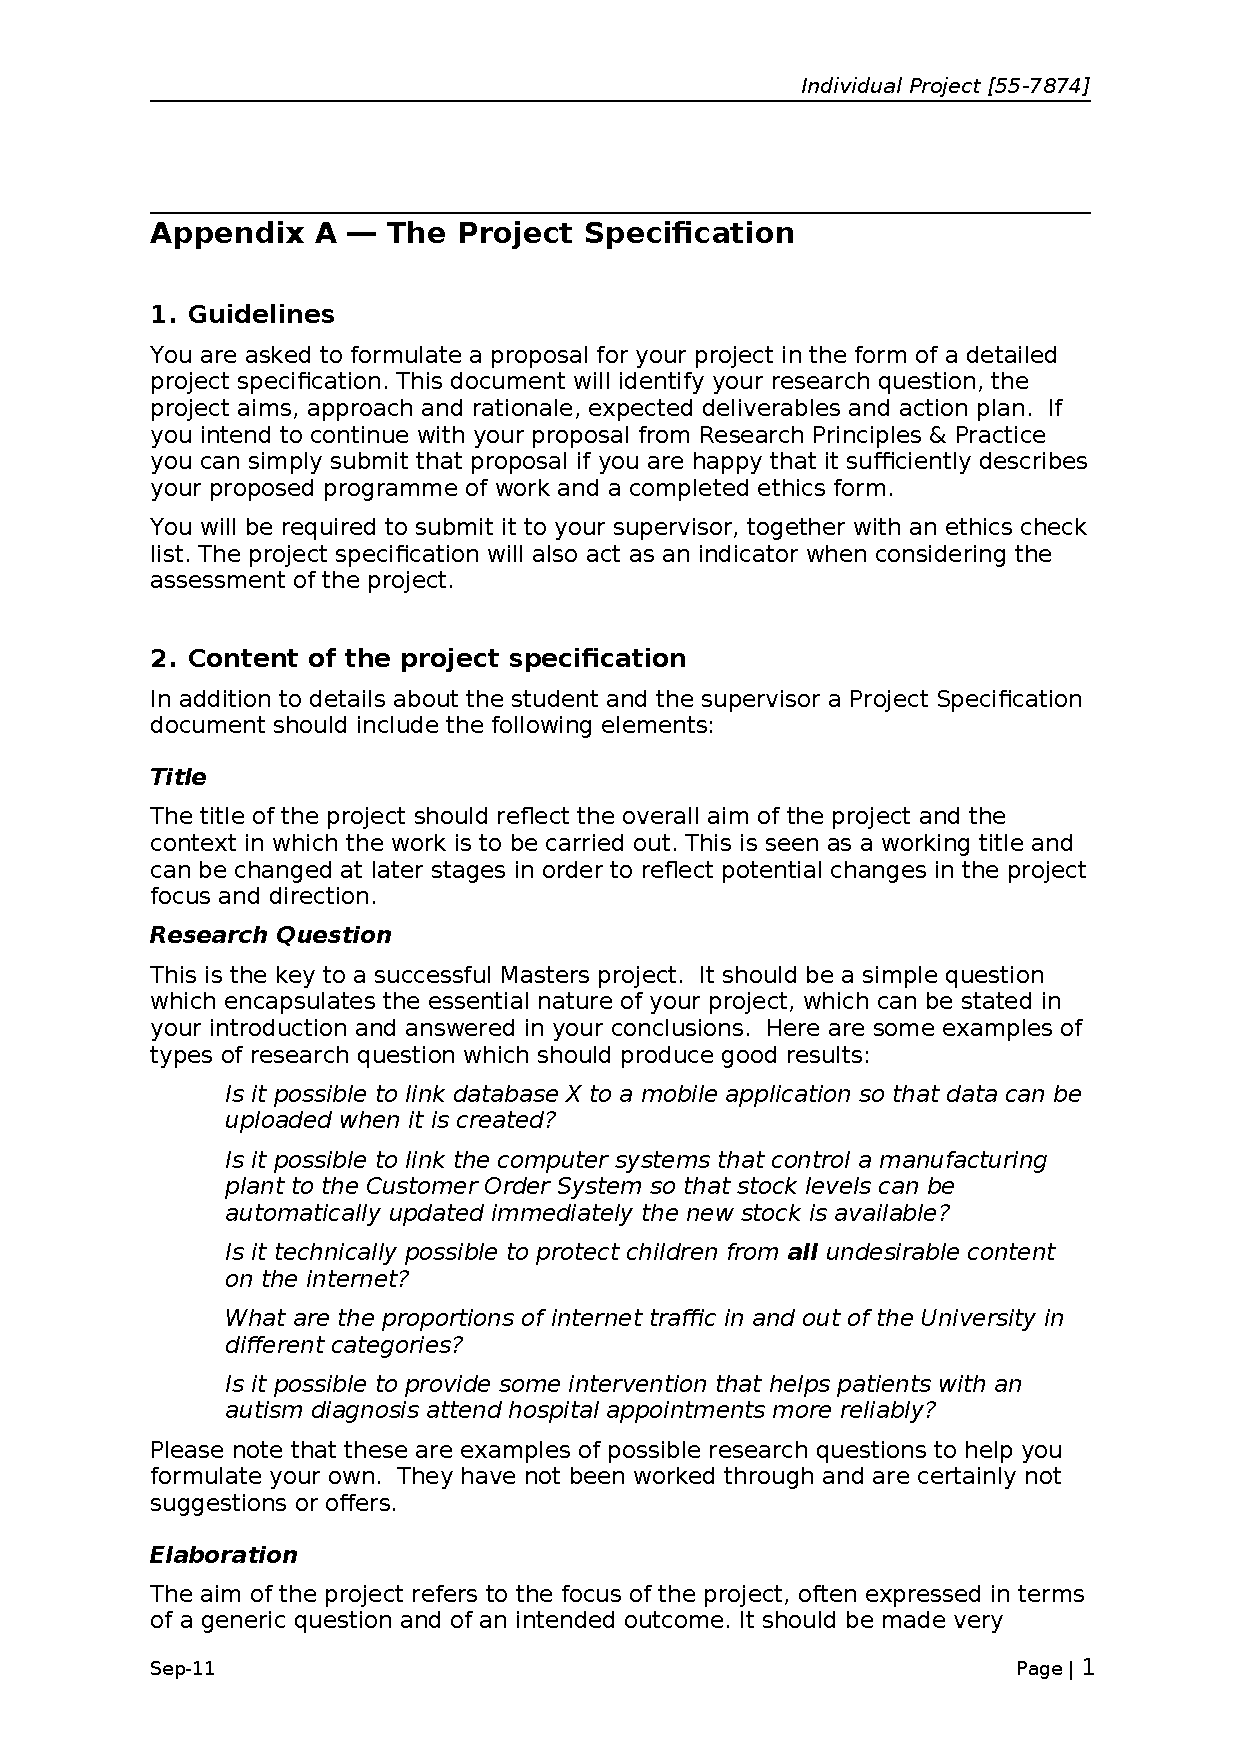
\includepdf[pages=-]{project_specification.pdf}

\chapter{Ethics}

\includepdf[pages=-]{ethics.pdf}

\includepdf[pages=-]{ethics_checklist.pdf}

\chapter{Methodologies for the development of software}
\label{appendix:softwareDevelopmentMethodologies}

\begin{description}

  \item[Waterfall:] Teams adopting the traditional waterfall method follow a rigid structure from planning to operations. Each step needs to be fully completed before moving on --- \citeauthor{royce1987managing} \parencite*[330]{royce1987managing} shows that a waterfall process is flawed when revisiting previous steps is required to finish the process. The waterfall methodology is easy to understand, but lacks the flexibility of other methodologies.

  \item[Rapid Application Development:] RAD was designed to be an improvement to the rigid structure of the waterfall method that can be considered a hindrance on some projects. RAD concentrates on having a fast, low-cost development of high-quality products \parencite{martin1991rapid}. RAD is typically used throughout the entire lifecycle of software \parencite[211]{beynon1999rapid}. This means that, to RAD methods, that the delivery and the development costs are just as important as the development itself. This project isn't concerned about development costs or a particularly fast delivery, and so the majority of the practices of RAD will be redundant.

  \item[DevOps:] The DevOps methodology focuses on the deployment of software, not the development. DevOps encourages short and continuous releases for software with each release being planned, programmed and built based on the feedback from the previous \parencite{bass2015devops}. This research isn't releasing anything to an external party and therefore does not benefit from the DevOps methodology, however, one thing to note is that "DevOps emphasizes the relationship of DevOps practices to agile practices" \parencite[15]{bass2015devops}, meaning that it is common for teams using DevOps to also use agile methods during development.

  \item[Agile:] According to The Agile Manifesto \parencite[2]{fowler2001agile}, agile methods embrace responding to change as opposed to how waterfall's planning process is there to avoid changes. Agile also places emphasis on people, whether they are developers or clients, collaborating on a regular basis to review and deliver parts of a project during development \parencite[3]{fowler2001agile}. There are frameworks like SCRUM \parencite[1]{fowler2001agile} that embody these same values, but being agile is about the team's recognition of these values and commitment to following them --- any approach can be agile as long as these values are remembered.

\end{description}

\chapter{Generic A* implementation}
\label{appendix:genericAStarImplementation}

\linespread{0.8}
\begin{lstlisting}[language=C++]
// A functor for using AStar
// Templates: thought STATE, ACTION, decision COST
template <class S, class A, class C>
struct AStar {

public:

  // Public getters
  const std::pair<A, C>& getCurrentAction() const { return currentAction; }
  const unsigned int& getStatesProcessed() const { return statesProcessed; }
  const std::vector<S>& getRemaining() const { return remaining; }
  const std::unordered_map<S, C>& getFScores() const { return fScore; }
  const std::unordered_map<S, C>& getGScores() const { return gScore; }

  // Evaluates options and returns a stack of actions to take
  std::pair<bool, std::stack<A>> operator() (
      const S& startingState,
      const C& minimumCost,
      const C& maximumCost,
      std::function<std::vector<A>(const S&)> getPossibleActions,
      std::function<bool(const S&, const S&)> isStateEndpoint,
      std::function<C(const S&)> heuristic,
      std::function<C(const S&, const S&, const S&, const A&)> weighAction,
      std::function<std::pair<bool, const S>(const S&, const A&)> takeAction,
      std::function<bool(const C&, const C&)> compareCost = std::less<C>()) {

    // All available states to explore
    remaining = {startingState};

    // Keep track of states already evaluated
    std::vector<S> evaluated = {};

    // Map of which action led to which thought state
    history.clear();

    // How much decision power gained so far in each state
    gScore = { { startingState, minimumCost } };

    // Map of predicted decision power from current state
    fScore = { { startingState, heuristic(startingState) } };

    // Keep track of the number of actions processed
    statesProcessed = 0;

    // Keep processing until there are no states left to check
    while (remaining.size() > 0) {

      // @ANALYSIS: Record how many moves have been processed
      statesProcessed += 1;

      // Get the highest priority state to operate on
      auto current = std::min_element(remaining.begin(), remaining.end(),
          [this, &maximumCost, &compareCost](const S& a, const S& b) {

        // Find fScores of a and b
        const C& fA = fScore.find(a) != fScore.end() ?
            fScore[a] : maximumCost;
        const C& fB = fScore.find(b) != fScore.end() ?
            fScore[b] : maximumCost;

        // Return whether fA should come before fB
        return compareCost(fA, fB);
      });

      // If we've arrived at a node that can be considered the goal, stop
      const S state = *current;
      if (isStateEndpoint(startingState, state)) {

        // Reconstruct the processes taken to get here
        S pathNode = state;
        std::stack<A> actionsTaken;

        // Build the path of actions from finish to start
        while (pathNode != startingState) {

          // Find how we got to the current state
          const auto& it = history.find(pathNode);
          if (it != history.end()) {

            // Get the data contained in the kvp
            const auto& previous = it->second;

            // Focus on the previous state for next iteration
            pathNode = previous.first;

            // Add action to the stack
            actionsTaken.push(previous.second);
          }

          // This shouldn't trigger as all routes should be traceable
          // However, if it does, stop the infinite loop
          else {
            assert(false);
            return std::make_pair(false, actionsTaken);
          }
        }
        return std::make_pair(true, actionsTaken);
      }

      // No longer consider the current state
      evaluated.insert(evaluated.end(), state);
      remaining.erase(current);

      // Initialise gScore of state if it's not there
      if (gScore.find(state) == gScore.end()) {
        gScore[state] = maximumCost;
      }

      // Get possible (neighbour) states by trying all possible actions
      const std::vector<A> actions = getPossibleActions(state);
      std::vector<std::pair<S, A>> states;
      std::for_each(actions.begin(), actions.end(),
          [&states, &evaluated, &state, &takeAction]
              (const A& action) {

        // Try taking the action with the current state
        const auto& attempt = takeAction(state, action);

        // Consider any valid states that haven't been evaluated
        if (attempt.first
            && std::find(evaluated.begin(), evaluated.end(), attempt.second)
                == evaluated.end()) {
          states.insert(states.end(), std::make_pair(attempt.second, action));
        }
      });

      // For each neighbour
      std::for_each(states.begin(), states.end(),
          [this, &startingState, &state,
          &maximumCost, &weighAction, &heuristic, &compareCost]
              (const std::pair<S, A>& future) {

        // Initialise gScore of neighbour if it's not there
        if (gScore.find(future.first) == gScore.end()) {
          gScore[future.first] = maximumCost;
        }

        // Work out cost of taking this action with the current state
        const C tentative_gScore = gScore[state] +
            weighAction(startingState, state, future.first, future.second);

        // @ANALYSIS: Record what the action is
        currentAction = std::make_pair(future.second, tentative_gScore);

        // If our projected score is better than the one recorded
        if (compareCost(tentative_gScore, gScore[future.first])) {

          // Record how we got to this node (insert new state and the action)
          history.insert(std::make_pair(
                future.first,
                std::make_pair(state, future.second)));

          // Update the gScore to the lower score
          gScore[future.first] = tentative_gScore;

          // Update fScore to a more accurate representation
          fScore[future.first] = tentative_gScore + heuristic(future.first);

          // If the current future isn't queued to be evaluated next, add it
          if (std::find(remaining.begin(), remaining.end(), future.first)
              == remaining.end()) {
            remaining.insert(remaining.end(), future.first);
          }
        }
      });
    }

    // Return unsuccessfully with the current state
    return std::make_pair(false, std::stack<A>());
  }

private:

  // All available states to explore
  std::vector<S> remaining;

  // Store FScores (costs of finishing pathing of all states)
  std::unordered_map<S, C> fScore;

  // Accurate cost of getting to a state
  std::unordered_map<S, C> gScore;

  // Map of which action led to which thought state
  // Map<future State, Pair<previous State, Action taken>>
  std::unordered_map<S, std::pair<S, A>> history;

  // Keep track of the number of actions processed
  unsigned int statesProcessed = 0;

  // Keep track of the current Action and its Cost
  std::pair<A, C> currentAction;

};
\end{lstlisting}
\linespread{1.5}

\chapter{Strategy game maps}
\label{appendix:strategyGameMaps}

\section{Default 5x5 map}
\label{sec:mapDefault5x5}

Figure \ref{fig:mapDefault5x5} shows the default map. 5x5 is big enough for basic play but small enough to keep processing fast. A good gauge of how well the AI performs is how well it copes with bigger map sizes, but 5x5 is the base requirement to be considered worth investigating. Teams on this map start with 5 MP and 3 AP per turn.

\begin{figure}[!h]
  \centering
  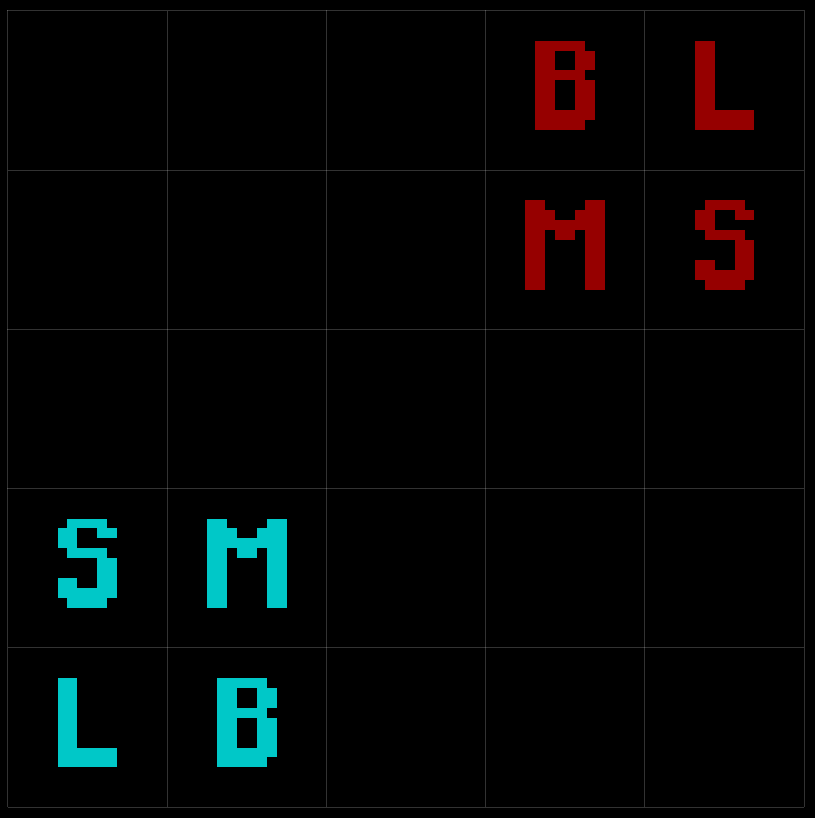
\includegraphics[width=10cm]{img/map_default_5x5.png}
  \caption{A symmetrical, 5x5 square map}
  \label{fig:mapDefault5x5}
\end{figure}

\pagebreak
\section{Cross-wall 5x5 map}
\label{sec:mapCrossWall5x5}

Figure \ref{fig:mapWithCrossWalls5x5} shows the default map with an orthogonal cross placed in the centre. This cross obstructs line of sight and the AI must attack the walls to remove them and attack the enemy. This map requires teams to do more \emph{Actions} to win, and therefore requires multiple turns to be beaten. Teams on this map start with 5 MP and 3 AP per turn.

\begin{figure}[!h]
  \centering
  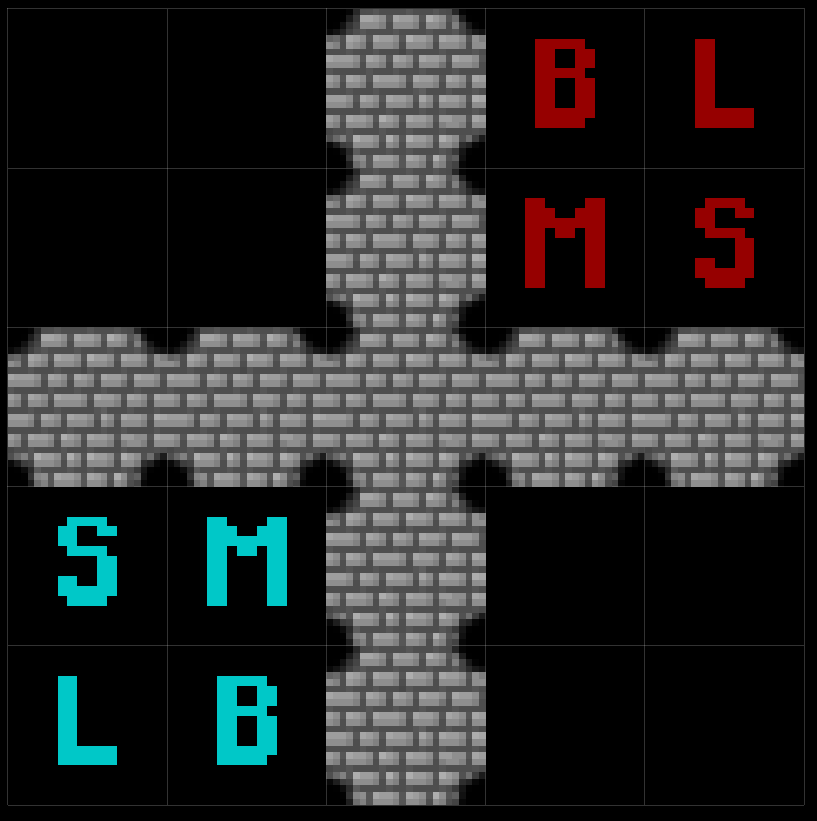
\includegraphics[width=10cm]{img/map_cross_wall_5x5.png}
  \caption{A symmetrical, 5x5 square map with obstacles dividing the map}
  \label{fig:mapWithCrossWalls5x5}
\end{figure}

\pagebreak
\section{Default 7x7 map}
\label{sec:mapDefault7x7}

Figure \ref{fig:mapDefault7x7} shows the default map. 7x7 is a big improvement than a 5x5 map but requires more resources to process. Recall that pathfinding is already an expensive process, so layering a lot of \emph{Actions} on top of all the possible movement possibilities means that the total number of nodes in a graph can easily go into the thousands. Teams on this map start with 5 MP and 3AP, this acts as a restriction that requires careful planning to work with.

\begin{figure}[!h]
  \centering
  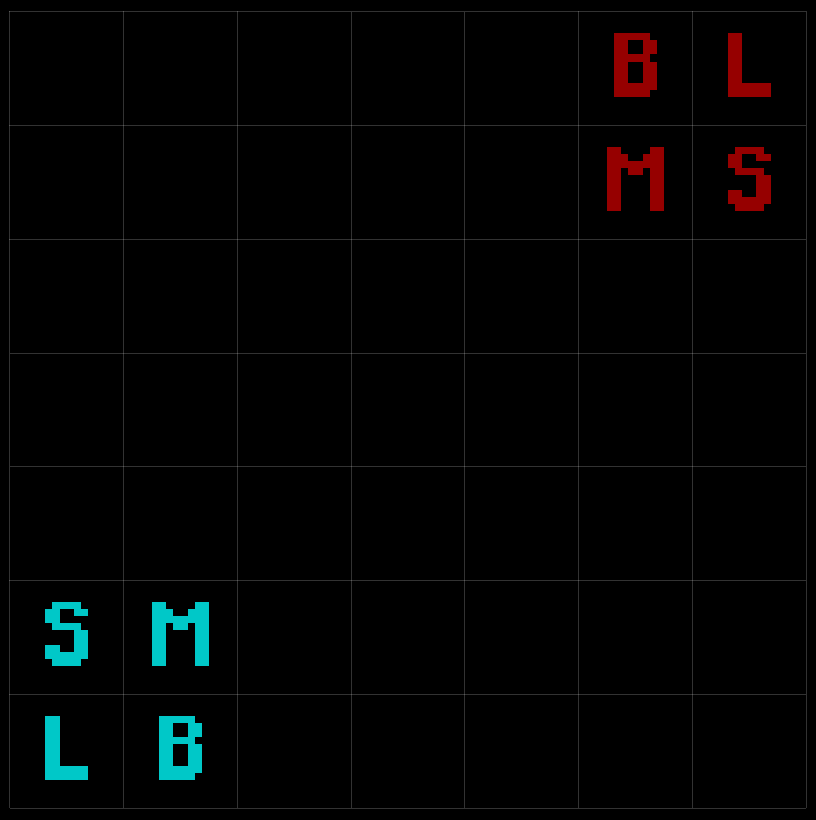
\includegraphics[width=10cm]{img/map_default_7x7.png}
  \caption{A symmetrical, 7x7 square map}
  \label{fig:mapDefault7x7}
\end{figure}

\pagebreak
\section{Cross-with-block 7x7 map}
\label{sec:mapCrossWithBlock7x7}

Figure \ref{fig:mapCrossWithBlock7x7} shows an extension of the map shown in section \ref{sec:mapCrossWall5x5}. The additional block in the middle makes going through the centre an alternative route to going around the sides. Teams start with 5 MP and 3 AP, making this map less about which team goes first and more about positioning and resources which is the true aim of the strategy game as noted in section \ref{subsec:designingStrategyGame}.

\begin{figure}[!h]
  \centering
  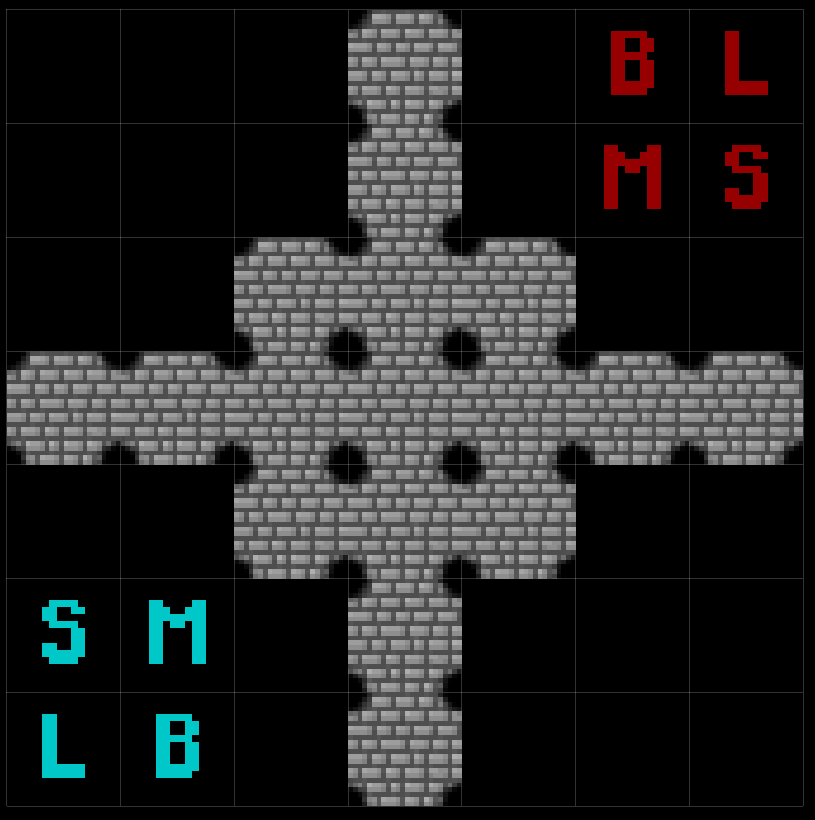
\includegraphics[width=10cm]{img/map_cross_with_block_7x7.png}
  \caption{A symmetrical, 7x7 square map with obstacles dividing the map}
  \label{fig:mapCrossWithBlock7x7}
\end{figure}

\chapter{Case study source code}
\label{appendix:caseStudySourceCode}

\section[Case one]{Case one (\emph{CaseOne.cpp})}
\label{sec:caseOneSourceCode}

\subsection{Weighing function}
\label{subsec:caseOneWeighingFunction}

\linespread{0.8}
\lstinputlisting[language=C++, firstline=61, lastline=134]
{../src/Scenes/Strategy/AI/CaseOne/CaseOne.cpp}
\linespread{1.5}
\pagebreak

\section[Case two]{Case two (\emph{CaseTwo.cpp})}
\label{sec:caseTwoSourceCode}

\subsection{Weighing function}
\label{subsec:caseTwoWeighingFunction}

\linespread{0.8}
\lstinputlisting[language=C++, firstline=80, lastline=160]
{../src/Scenes/Strategy/AI/CaseTwo/CaseTwo.cpp}
\linespread{1.5}
\pagebreak

\section[Case three]{Case three (\emph{CaseThree.cpp})}
\label{sec:caseThreeSourceCode}

\subsection{Weighing function}
\label{subsec:caseThreeWeighingFunction}

\linespread{0.8}
\lstinputlisting[language=C++, firstline=103, lastline=398]
{../src/Scenes/Strategy/AI/CaseThree/CaseThree.cpp}
\linespread{1.5}
\pagebreak

\section[Case four]{Case four (\emph{CaseFour.cpp})}
\label{sec:caseFourSourceCode}

\subsection{Goal function}
\label{subsec:caseFourGoalFunction}

\linespread{0.8}
\lstinputlisting[language=C++, firstline=147, lastline=196]
{../src/Scenes/Strategy/AI/CaseFour/CaseFour.cpp}
\linespread{1.5}
\pagebreak

\subsection{Heuristic function}
\label{subsec:caseFourHeuristicFunction}

\linespread{0.8}
\lstinputlisting[language=C++, firstline=198, lastline=266]
{../src/Scenes/Strategy/AI/CaseFour/CaseFour.cpp}
\linespread{1.5}
\pagebreak

\subsection{Weighing function}
\label{subsec:caseFourWeighingFunction}

\linespread{0.8}
\lstinputlisting[language=C++, firstline=268, lastline=335]
{../src/Scenes/Strategy/AI/CaseFour/CaseFour.cpp}
\linespread{1.5}
\pagebreak

\addtocontents{toc}{\endgroup}
\end{appendices}

\end{document}
